\section{Introduction}

% == The Challenge -> to raise importance for CNNs compression.
State-of-the-art Convolutional Neural Networks (CNNs) are becoming the go-to solution in computer vision for automated systems operating in complex high dimensional domains. 
%
Achieving high accuracy of CNN models during training usually come at the expense of overparameterizing the model~\cite{Neill2020}.
%
This results in well performing CNNs that are oversized. 
%
Being oversized hinders the deployment of CNN models on low-resource computers as well as having an unnecessary large carbon footprint during operation.
%
These issues are expected to get worse as the complexity of operational environments increase and thus the models will consequently need to be larger, making the deployment even more challenging~\cite{Marino2023, Brown2020}.  

% == Introduce Deep Neural Network Compression
A work around could be to take an adaptability approach, where a smaller model is trained on a subset of the operational environment and then one relies on adapting the model depending on shifts in the environment e.g.~\cite{Ghobrial2022, mirza2022norm}.
%
These approaches present their own questions regarding information forgetting, resource requirements and energy consumption.
%
Also, whilst this may assist with the problem of needing to increase the model size as the operational environment increases,
% increasing operational envionrnments deploying models on to low resource computers.
the neural network will still be oversized compared to the amount of information retained at one time. 

Therefore, \textit{neural network compression} has recently seen a surge in its research outputs, as compression offers significant reduction in size and energy consumption whilst retaining more or less the same overall accuracy performance and improving the speed of predictions. 
%
% == Brief overview on existing CNN compression techniques. Highlight on Quantisation and Pruning if adequate.
There are many compression techniques in the literature that fall under one of these compression categories: pruning, quantisation, knowledge distillation and tensor decomposition. These different categories are nicely discussed in these two reviews \cite{Neill2020}\cite{Marino2023}.
%
% == Elaborate on the need for standardisation between these techniques.
With all of the effort being put in developing different compression techniques, yet the community seems to lack a standardised way of evaluating different compression techniques.

  
% Goal of NEtzip is standardising evaluation of DNN Quantisation. Netzip also facilitates the usage of ShrinkBench is a standardisation library for pruning methods, which allows users to compare between pruning and quantisation techniques.  

% Unlike TensorFlow which may support integer quantization using arbitrary bit-width from 2 to 16, PyTorch only supports bit-widths of 8 according the this blog: \url{https://leimao.github.io/blog/PyTorch-Quantization-Aware-Training/}


% In our case study we focus on CNNs, however, in our future works we plan to extend this to include LSTMs transformers  etc. (use this link from pytorch to help categorise the different types of DNNs: https://pytorch.org/docs/stable/quantization.html\#general-quantization-flow)
% \subsection{Motivation}

% Why is it important to standardise?
Based on a recent review, most of the introduced methods in the literature available do not compare their introduced compression techniques with existing techniques and where comparisons are made they tend to vary between different publications~\cite{Blalock2020}.
%
This is largely due to the lack of standardised implementations of metrics, neural networks, compression techniques. 
%
In this paper, we focus predominantly on the metrics aspect.
%
The contributions of this paper are two folds: 
\begin{enumerate}
    \item Provide a review of evaluation metrics used to assess compression techniques. 
    \item Using the reviewed evaluation metrics, we introduce NetZIP, a growing standardized benchmark library for comparing compression techniques available at \url{https://github.com/TSL-UOB/NetZIP}. NetZIP is aimed to help users identify the most suitable compression technique for their trained neural network using several baseline compression techniques, and also serve to compare newly developed compression techniques against others.%some standard compression techniques and CNNs. 
\end{enumerate}
%

The paper is organised as follows, in section~\ref{sec:background} we overview compression methods and existing compression benches. We provide our review of evaluation metrics in section~\ref{sec:metrics}. Section~\ref{sec:NetZIP_overview} introduces NetZIP and section~\ref{sec:casestudies} showcases comparisons made using NetZIP. Conclusions and futures work are provided in section~\ref{sec:Conclusions}.

\begin{figure*}
    \centering
    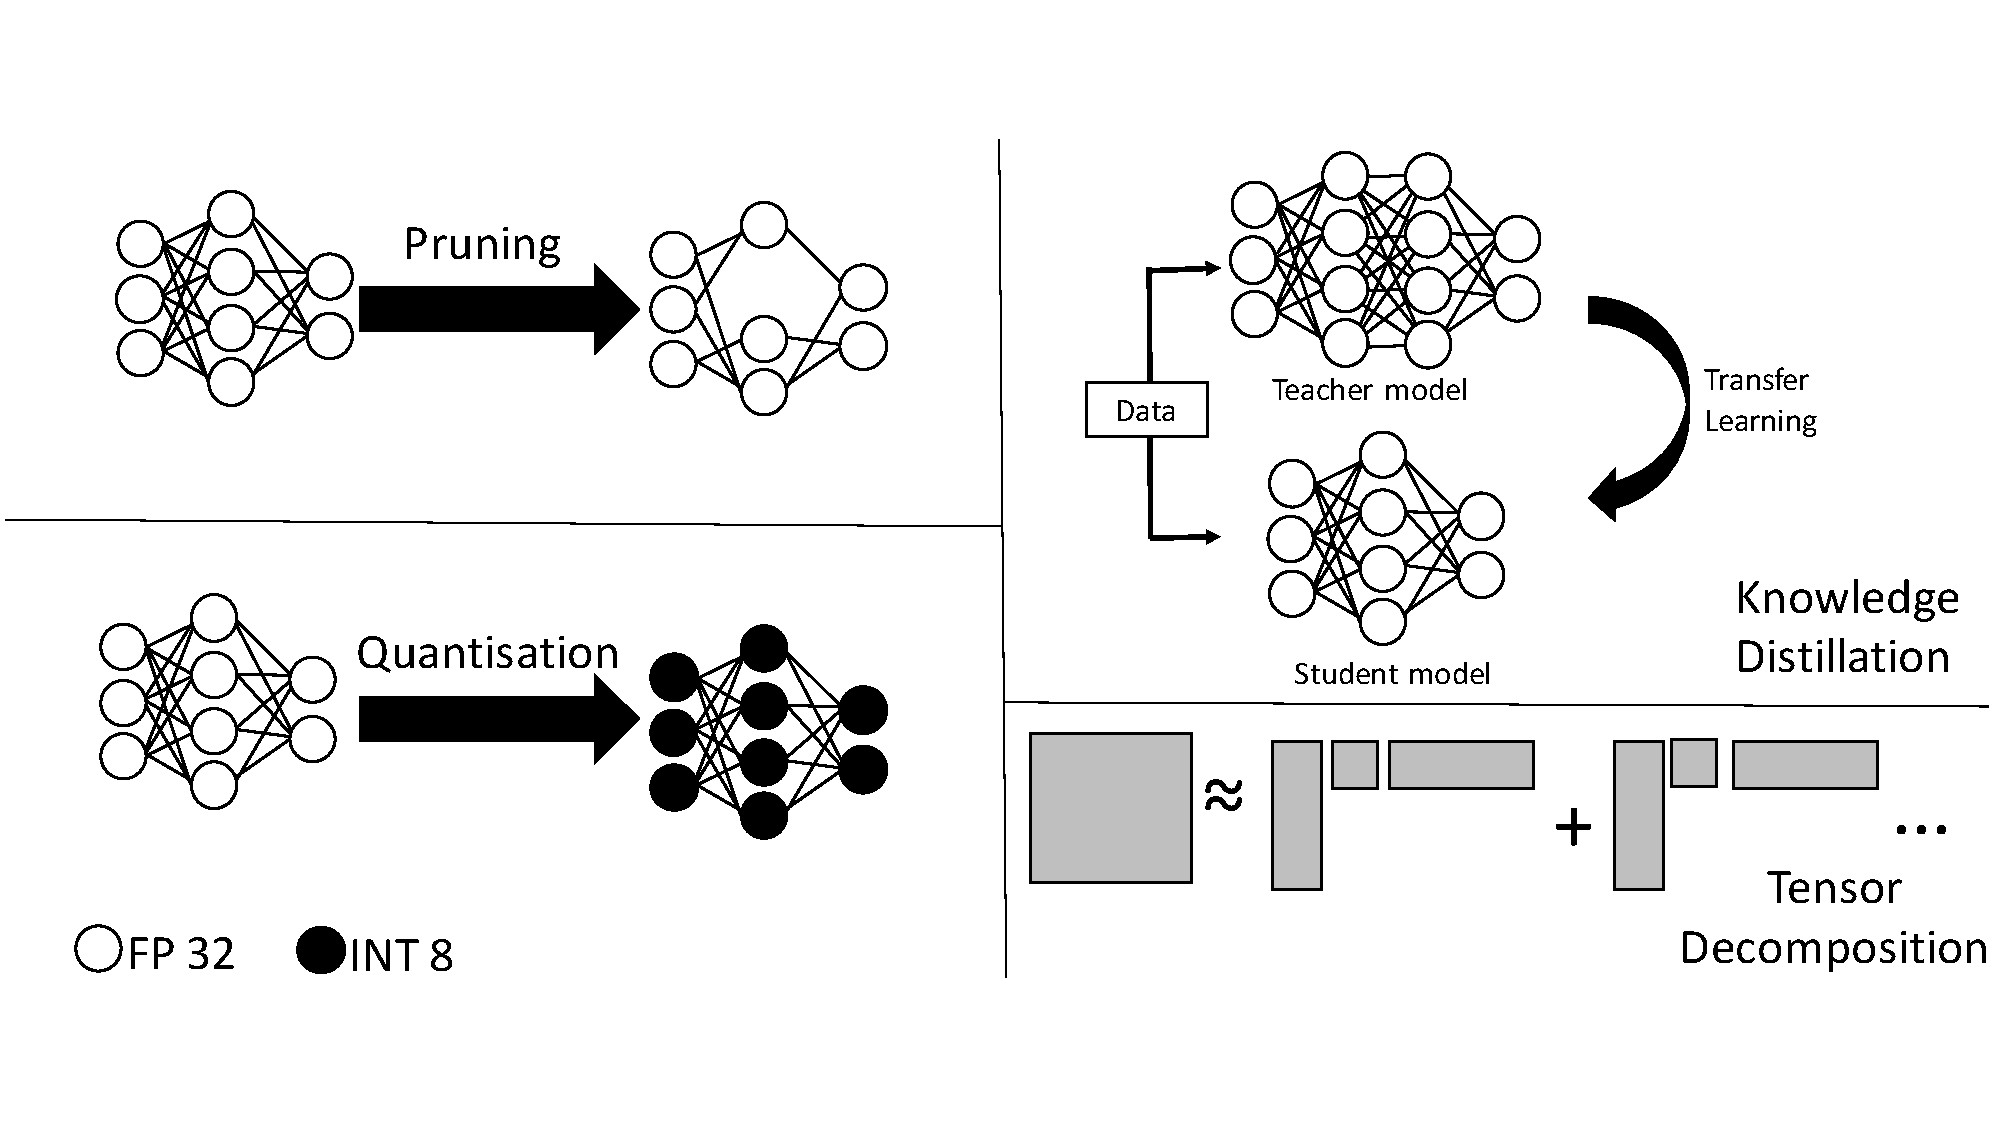
\includegraphics[width=1\textwidth]{other/figures/compression_methodsv2.pdf}{}
    \caption{Shows an overview of the four compression techniques categories currently available in the literature. The four categories are Pruning, Quantisation, Knowledge Distillation and Tensor Decomposition.}
    \label{fig:compression_methods}
\end{figure*}

% Why compression? 

% -Decreases model size.

% -Decreases energy consumption.

% -Increases Speed.

% Reduced computational requirements: Smaller models require fewer resources to train and deploy, which can significantly reduce the computational requirements and energy consumption.

% Improved memory and storage efficiency: Smaller models require less memory and storage space, which can be particularly useful in scenarios where resources are limited, such as mobile devices or edge computing.

% Faster inference: Smaller models can perform inference faster, which is particularly important in real-time applications such as object detection and autonomous driving.


% Why standardised compression bench.
% Effectiveness of compression can vary due to~\cite{Blalock2020}:
% Blalock et.al.~\cite{Blalock2018} 

% -Variations in initializations. 

% -Initial model training.

% -Different Implementation of deep learning libraries.
% \subsection{Contribution and Organisation of paper}




% =====

% Whilst NetZIP is meant to be a growing toolkit library, currently we currently focus on deep neural networks for vision tasks, with the scope of expanding to natural language processing applications and other fields needed by the community. 

% NetZIP is an open-source bench marking framework for evaluating the performance of model compression techniques on deep neural networks. It provides a standardized set of benchmarks and evaluation metrics for comparing different compression methods.
%
% NetZIP allows for training models from scratch or using pre-trained models  to evaluate compression techniques. It also includes a suite of compression methods, mainly pruning and quantization, which can be easily applied to the pre-trained models.
%
% The framework provides a range of evaluation metrics to measure accuracy, speed, size, and energy which can be used to assess the performance of the compressed models. 
%
% NetZIP is designed to be easily extensible, allowing researchers and developers to add their own models and compression techniques to the benchmarking suite. 
% Overall, NetZIP provides a standardized framework for evaluating the performance of model compression techniques, enabling researchers and developers to more easily compare and evaluate different methods.



% \begin{enumerate}
    % \item Identify the most suitable compression technique for their trained Neural Network using several (baseline) compression techniques.
    % \item Compare newly developed compression techniques against some standard compression techniques and CNNs.
% \end{enumerate}

% Mention that this compression bench is in continuous development and will continue to evolve over time. 

% \section{Definitions (~0.5 pages)}


\section{Background} \label{sec:background}

% \begin{figure*}
%     \centering
%     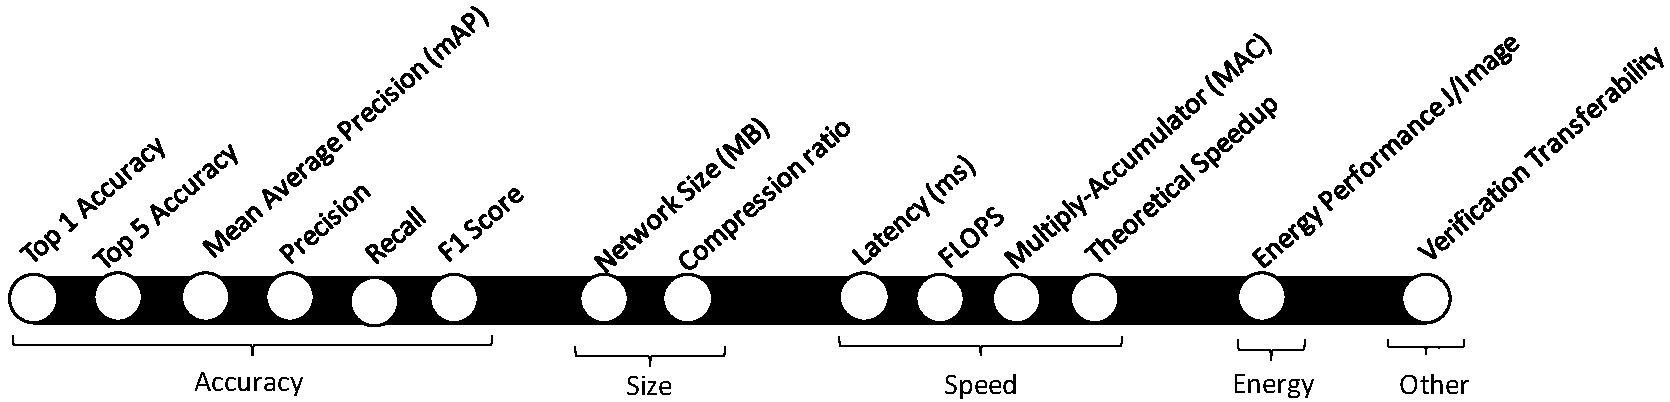
\includegraphics[width=1\textwidth]{other/figures/metrics.pdf}{}
%     \caption{Metrics}
%     \label{fig:metrics}
% \end{figure*}

In this section we cover a high-level overview of compression methods and we discuss existing compression benches.% and how NetZIP compliments and extends existing works.

\subsection{Compression Methods Overview}
Following Neill et.al.~\cite{Neill2020} and Marino et.al.~\cite{Marino2023} overviews, compression techniques are broken into four categories shown in Figure~\ref{fig:compression_methods} and briefly explained below:
\begin{enumerate}
    \item \textit{Pruning:} Requires the scanning and removing of neurons and connections that does not have a significant influence on the output prediction of the neural network.

    \item \textit{Quantisation:} Aims at reducing the numerical representation of values in a neural network model, for example by converting values expressed in a neural network from single-precision 32-bit floating point (FP32) numbers to 8-bit integers (INT8).

    \item \textit{Knowledge Distillation:} Trains a large neural network (teacher model) on a dataset. Then a smaller neural network (student model) is trained on the same dataset whilst guided by the teacher model through transfer learning techniques to help the student model optimise achieving similar accuracy as the teacher model.

    \item \textit{Tensor Decomposition:} Involves the decomposition of large weight tensors by approximating them to additions and products of lower order tensors.
      
\end{enumerate}
% \subsubsection{Pruning}
% Involves scanning and removing of neurons and connections that does not have a significant influence on the accuracy performance of the neural network.

% \subsubsection{Quantisation}
% Aims at reducing the precision of numerical values in a neural network model, for example by converting values expressed in a neural network from single-precision 32-bit floating point (FP32) numbers to 8-bit integers.

% \subsubsection{Knowledge Distillation}
% Trains a large neural network (teacher model) on a dataset. Then a smaller neural network (student model) is trained on the same dataset whilst guided by the teacher model through transfer learning techniques to help the student model optimise achieving more or less the same performance as the teacher model. 

% \subsubsection{Tensor Decomposition} Involves the decomposition of large weight tensors by approximating them to additions and products of lower order tensors.



% ==== Useful notes that might be worth keeping =====
% Survey \cite{Gholami2022}, \cite{Liang2021}

% Useful link that provides tips on deployment after quantisation and what you need to be aware of: https://spell.ml/blog/pytorch-quantization-X8e7wBAAACIAHPhT

% Paper that mentions one should avoid quaantising the first and last layer in a DNN https://arxiv.org/pdf/1603.05279.pdf
% ===================================


\subsection{Compression Benches}
Creating benches for standardising neural network compression is currently a growing area of research. %
%
Microsoft Neural Network Intelligence (Microsoft NNI)~\cite{nni2021} is an open-source toolkit that helps users automate the optimization of deep learning models. It supports different deep learning frameworks mainly PyTorch and TensorFlow, allowing users to easily run experiments for optimising their models. 
%
One of the core parts of Microsoft NNI toolkit is model compression. They provide a growing library of compression techniques available in the literature, such as~\cite{courbariaux2016binarized, esser2020learned, yang2022oneshot, frankle2019lottery}, making it accessible and efficient for users to experiment using state of the art compression techniques. Microsoft NNI also provides a web-based dashboard to track and visualize the results of experiments.
%
However, the toolkit does not dive into standardisation nor provides a comprehensive set of metrics for standardising the evaluation of neural network compression.

Blalock et.al.\cite{Blalock2020} tried to solve the lack of neural network compression standardisation in the community by analysing a large number of literature and generated a catalog of common issues in comparisons of compression techniques.
%
This was summarised into a set of best practices to mitigate these issues. Using these best practices they implemented ShrinkBench, a standardised library for comparing between neural network pruning methods. 
%
% In summary these best practices are summarised here: 1) start from the same initial model 2) Compare accuracy and theoretical speed up for the same compression ratio, as different compression ratios may result in which compression technique is best....  
%
We take into account the best practices summarised by Blalock et.al.\cite{Blalock2020} when carrying out our experiments using NetZIP. 
%
NetZIP is also a standardised compression bench but aimed at providing a comprehensive set of metrics for evaluating deep neural networks compression techniques. The need for such a tool standardising metrics for compression as been pointed out implicitly by Blalock et.al. 

Facebook research provides some relevant evaluation metrics for neural networks as part of their \textit{Slowfast}~\cite{fan2020pyslowfast} repository implementation. Whilst the metrics provided are not comprehensive for compression methods evaluation, yet it has provided some insight in the course of development of our paper.

An issue relevant to the context of our paper is the difficulty in generalising the removal of zeroed parameters from different pruned neural network architectures. For example, current implementations of pruning in PyTorch sets a value of zero to the pruned parameters but does not automatically remove the zeros from the network structure. This is because removing structural parameters from a neural network can result in malfunctioning of the network and generated errors. 
%
Hence, removing the zeroed parameters currently rely on manually designing case-dependent schemes that do not generalize to different neural network architectures. 
%
Developing a method for generalising and automating the removal of these parameters is beyond the scope of our paper. 
% but we use the sparsity level to provide an evaluation of the compression in size as will be discussed later in the paper. Removing the zeroed parameters is case-dependent, 
We direct interested readers towards DeGraph~\cite{fang2023depgraph} which aims at generalising the the approach of removing pruned parameters invariant of the architecture. 
%


%
% However, not being able to remove the pruned parameters stops us from evaluating benefits on model size from compression after pruning. We suggest


% Another interesting related work is DepGraph~\cite{fang2023depgraph}, which dives into the issues uctural pruning enables model acceleration by removing structurally-grouped parameters from neural net- works. However, the parameter-grouping patterns vary widely across different models, making architecture- specific pruners, which rely on manually-designed grouping schemes, non-generalizable to new architectures. In this work, we study a highly-challenging yet barely-explored task, any structural pruning, to tackle general structural pruning of arbitrary architecture like CNNs, RNNs, GNNs and Transformers. The most prominent obstacle towards this goal lies in the structural coupling, which not only forces different layers to be pruned simultaneously, but also expects all removed parameters to be consistently unimpor- tant, thereby avoiding structural issues and significant per- formance degradation after pruning.



% Current implementations of pruning PyTorch only aims at zeroing the pruned parameters but does not remove these parameters from the tensors, therefore the actual size of the saved model does not decrease. Sparsity can be a representative of Compression ratio for pruning. However, efforts are currently being devoted into creating libraries that 


% \cite{Babaeizadeh2016} propose NoiseOut, a fully automated pruning algorithm based on the correlation between activations of neurons in the hidden layers.

% \cite{Zhou2019a}




% \cite{Yang2019}

% Larqx



\section{Metrics}\label{sec:metrics}
In this section we overview different assessment metrics that serve the evaluation of networks models and compression techniques. For each metric we discuss how it can be computed and the information it provides for assessment. We break the evaluation metrics into five categories: Accuracy, Size, Speed, Energy and Other; each category has different evaluation metrics (see Table~\ref{tab:metrics_summary}).

\setlength{\arrayrulewidth}{0.1mm}
\setlength{\tabcolsep}{2pt}
\renewcommand{\arraystretch}{1.75}
\begin{table*}[]
    \centering
    \begin{tabular}{| c | l l l l l |} 
        \hline
        Category &  & & Metrics & &  \\
        % \multicolumn{5}{1}{Metrics} \vline \\
        \hline
        Accuracy & Top-k Accuracy &  Precision & Recall & F1-Score & Mean Average Precision \\ 
        Size     & Disk Size &  Parameters Count & CPU usage & GPU usage &  \\  
        Speed    & Inference Latency &  Number of Operations & MACs & FLOPs &   \\ 
        Energy   & Power &  Energy &  &  &  \\ 
        Other    & Compression Ratio & Speedup Ratio &  Efficiency Ratio &  & \\ 
        \hline
    \end{tabular}
    \caption{Metrics Summary}
    \label{tab:metrics_summary}
\end{table*}

\subsection{Accuracy}
\subsubsection{Top-k Accuracy}
Top-k accuracy is used to measure the accuracy of a model.%, often used in the context of object classification.
%
Top-k accuracy shows the proportion of test samples for which the most likely $k$ predicted class labels match the ground truth class label, where $k \in \{1, ...,  K\}$ and $K$ is the max number of classes in the model being evaluated.
%
Two commonly used values for $k$ are 1 and 5. Top-1 accuracy in this case will only consider a prediction correct if it matches the ground truth label, whilst Top-5 accuracy will consider a prediction correct if one of the top 5 predictions of the model output matches the ground truth label. 

Top-k accuracy, for $k>1$, can be particularly useful where the model has a large number of classes, with several classes being similar to each other. 
%
In this case it may be challenging for the model to accurately predict the correct class, but for example a prediction amongst the top three possibilities may still be helpful.

\subsubsection{Precision}
Precision is a measure of the accuracy of the predictions output by a model, which aims at conveying how many of the predictions are accurate out all predictions. 
%
In other words, precision is the fraction of predictions that are true positives (TP), i.e. correctly identified objects out of all the predictions made by the model, including both true positives and false positives (FP),i.e. objects incorrectly identified (see equation~\ref{eq:precision}).
%
In the context of object classifications TP and FP are counted by simply matching the predicted label with the ground truth label. 
%
In object detection the intersection over union (IoU) is calculated as the ratio of overlap between the ground truth annotations and the output predictions. If the IoU passes a certain chosen threshold, then the prediction is counted as TP. 
\begin{equation}
  Precision =   \frac{TP}{TP+FP}
  \label{eq:precision}
\end{equation}


% \begin{equation}
%     AP = \frac{1}{N} \sum_{i=1}^{N} AP_i
% \end{equation}

% \begin{equation}
%     mAP = \frac{1}{N} \sum_{i=1}^{N} AP_i
% \end{equation}

\subsubsection{Recall} On the other hand, \textit{recall} is a measure that expresses the rate of a model getting correct predictions.
% Is a measure of how well a model is able to identify all instances of a particular object class within an image or a set of images. 
Specifically, recall is the fraction of true positive predictions, out of all present instances in the test sample  i.e. true positives + false negatives (FN), see equation~\ref{eq:recall}.
% Recall is an important measure in object detection, as it helps to ensure that a model is not missing any instances of a particular object class. However, it should be used in conjunction with other metrics, such as precision and mean average precision (mAP), to provide a more complete evaluation of the performance of an object detection model.

\begin{equation}
  Recall =   \frac{TP}{TP+FN}
  \label{eq:recall}
\end{equation}

\subsubsection{F1 Score}
The F1 score is a metric that combines both precision and recall into a single metric. The F1 score is the harmonic mean of precision and recall, given by equation~\ref{F1_score}.
%
The F1 score provides a way to balance the trade-off between precision and recall, as both measures are important for different aspects of model performance. A high F1 score indicates that a model has both high precision and high recall, meaning that it is able to correctly identify a high percentage of positive instances whilst also minimizing the number of false positives.

\begin{equation}
  \text{F1 Score} =   \frac{2 \cdot \text{Precision} \cdot \text{Recall}}{\text{Precision} + \text{Recall}}
  \label{F1_score}
\end{equation}

\subsubsection{Mean average precision (mAP)}
Mean average precision (mAP) is a metric that takes into account both precision and recall of a model. 
%
The metric is calculated by summing the average precision ($AP$) of each class $k$ over the number of classes $K$, as shown by equation~\ref{eq:mAP}.  
% of the the mean of the different average precision for different classes as shown by equation~\ref{eq:mAP}

\begin{equation}
    mAP = \frac{1}{K} \sum_{k=1}^{k=K} AP_k
    \label{eq:mAP}
\end{equation}
The AP of each class is calculated by plotting precision for different recall values and calculating the area under the curve (AUC). To plot the precision-recall graph an intersection over union (IoU) threshold needs to be selected. In the case where an optimal IoU threshold is not selected or unknown, then the AUC can be calculated for several IoU thresholds and averaged to give an AP representative of a range of IoU thresholds.  

Compared to F1 Score, mAP is more sensitive to imbalances in the number of training samples between different classes, whilst the F1-score is insensitive to these imbalances in training samples. On the other hand mAP is more expensive to compute compared to the F1 Score.
%
When the model is at the stage of training, mAP is a more informative metric to use in assessing the performance of the model on different prediction classes. 
%
However, in comparing between compression techniques the F1 score may be a more efficient metric for carrying out an initial assessment to identify best compression techniques. A thorough analysis using mAP may still be required dependent on the application context.


% This shows that the AP metric is dependent on the IoU threshold. Choosing the IoU threshold becomes an arbitrary process for the researcher as it needs to be carefully chosen for each task as the model's accuracy expectation may vary. Hence, to avoid this ambiguity while evaluating an object detection model, the mean average precision(mAP) came into existence.
%
% The metric is calculated by computing the precision for different levels of recall, by varying the threshold for how confident a model needs to be in order to consider a prediction as positive. The area under the curve (AUC) for the precision-recall curve plot is computed.
%
% The mAP is the average of the area under the curve  values for each class

% is then plotted, and the area under the curve (AUC) is calculated. The mAP is the average of the AUC values for each class of object being detected. A high mAP indicates a model that produces accurate and reliable predictions across a range of recall levels, and is often used to compare the performance of different object detection models.

% In the context of compression, the model being compressed is usually trained to there may be less emphasis on training balance  
% The mAP for object detection is the average of the AP calculated for all the classes. mAP@0.5 means that it is the mAP calculated at IOU threshold 0.5... %usefull link -> %https://www.kdnuggets.com/2020/08/metrics-evaluate-deep-learning-object-detectors.html

% The difference between mAP and F1 score is that the F1 score is a single value that provides an overall evaluation of the balance between precision and recall in a classification task, while mAP is a more detailed evaluation metric that is used in object detection tasks to measure the accuracy of detection for different object classes.

\subsection{Speed}
\subsubsection{Inference Latency}
Is the time taken for the model to output its prediction of the input. 
%
Whilst latency may give the most practical real-time value for operation speed estimates and machine specific comparisons, it is affected by resource utilisation of the machine at the time of measurement. 
%
This makes the measured time variant to the level of resource utilisation, thus may be less informative about the benefit of compression in some cases, especially if experiments are run on different machines or at different times where the level of resource utilisation may vary. 
%
This is analogous to an issue of variance in generated test results caused by resource utilisation changes in simulation based testing~\cite{determinisim}.
%
In cases where the resource utilisation is known to have significant variations, one may resort to counting the number of operations or analysing the different proportions of numerical representation in the model after compression to deduce signs of speed improvement.%, analysing the different portions of numerical representation in the model, or observing the reduction in disk size after compression to deduce signs of speed improvement. 
%
These other metrics may be useful when comparing between different compression algorithms within the same category of compression (e.g. pruning only or quantisation only) but may suffer from providing useful information when comparing between different compression categories. 
%
This is discussed further below, however, during carrying out our experimentation, we found that controlling the resource utilisation and using inference latency as a metric is the best way to quantitatively compare improvements in speed between different compression categories.

% or comparisons are being made between compression techniques ran on different machines, one may resort to counting the number of operations or  


% a more informative measure to report improvement on speed can be %MACs or FLOPs, which effectively 
% to count the number of operations undertaken to output a prediction as a measure of speed, discussed in more detail below. 


\subsubsection{Number of Operations}
Computing the total number of operations for a neural network to output a prediction can be another way of measuring the improvement in speed gained by compression. 
%
This is especially useful when carrying out experiments on different machines or if resource utilisation varies between different experiments run on the same machine. 
%
For quantisation techniques, however, only the numerical representation type changes in the neural network but the number of parameters stay the same in the model. 
%
Even though quantisation does provide improvement in speed, calculating the number of operations may not provide any insight of that, as the number of operations count will be the same pre- and post-compression. 
%
For other compression techniques like pruning for example where parameters are removed from the model, measuring the number of operations can be an insightful metric for evaluating speed improvements.

Floating-Point Operations (FLOPs) is a popular metric in measuring the speed improvement in compression literature especially for pruning. FLOPs only takes into account floating points operations. 
%
Therefore, for quantisation techniques where the parameters are not of type float, not all operations will be counted. This may convey inaccurate estimations of speed improvements when comparing between quantisation and pruning techniques. Nevertheless, observing proportions of different types of numerical representations may give insights of speed improvements.  
%
% Yet measuring if there any floating points operations existing in a quantised model may give indicative signs of speed improvements for quantisation, as noticed in the experimental case studies section discussed later. 
%
% From this observation, an interesting area of research is to find if there can be an analytical or empirical correlations between speed improvements and proportions of different numerical representation types involved in a compressed neural network.  


Multiply-Accumulator Operations (MACs) is another commonly used metric to count operations that involve all types of numerical representations i.e. not only floats. There are not any obvious advantages, as far as we are aware, of using MACs over the total number of operations referred to earlier. Perhaps the main strength of using MACs is its popularity over total number of operations. One MAC is defined as containing one multiplication and one addition operations, therefore MACs can be calculated as the total number of operations divided by two. 

\subsection{Size}
\subsubsection{Disk size}
The space required to keep the model on a computer can be of significance especially when models are large e.g. ChatGPT-3~\cite{Brown2020}. Compression techniques can help in significantly reducing the model size so less disk space is required. For example quantisation of model parameters from FP32 to INT8 numerical representation decreases disk size required to save the model typically by a quarter. 
%



% - discuss point on sparsity here as well

 

\subsubsection{Parameters Count}
Another way of measuring the size of the model is by counting the number of parameters in the compressed model compared to the uncompressed version. This method can be useful when comparing compression techniques where parameters are actually removed from the model e.g. pruning. 
%
The usefulness of parameters count will fall short when it comes to quantisation techniques, where the number of parameters stay the same but the numerical representation changes.
In these cases using the disk size as a metric to compare between compression techniques can be a more informative measure than parameters count.

Nevertheless parameters count can be of great use at early stage assessment of pruning techniques.
%
In many of the popular pruning libraries implementations e.g. PyTorch~\cite{paszke2017automatic}, typically the pruned parameters are zeroed but not removed from the model.
%
This is due to errors likely to occur when structural parameters are removed in pruning. Removing the zeroed parameters from the architecture is currently an active area of research e.g.~\cite{fang2023depgraph}, as currently removing the pruned parameters is a manual and custom process reliant on the model architecture. 

Therefore, non-zeroed parameters count can serve to show how much reduction in disk size will be achieved using different pruning techniques, prior to committing to the manual process of removing pruned parameters. 
%
Furthermore, the proportion of the uncompressed model parameters which are zeros after compression is known as \textit{sparsity}.
% ratio of zeroed parameters over the tota metric derivative of parameters count showing what 
% Note: Due to errors likely to occur when structural parameters are removed inp pruning as discussed earlier in our related work section, we use the sparsity in the neural network to measure the size/compression ratio.

\subsubsection{CPU/GPU usage}
Measuring the reduction in computational resources used by the model to output a prediction is another important factor to assess when investigating the trade-offs between different compression techniques.
%
This becomes of interest in applications where onboard processing resources are limited and critical to the survival of the system. 
%
%
% Measuring CPU and even GPU useage can be achevied ....

% ========================

% The two types memory of most relevance for neural network compression evaluation are, random-access memory (RAM) and storage memory such as hard disk drives (HDDs) and solid-state drives (SSDs).
% %
% RAM is used to store data and instructions that the computer is currently using. 
% %
% Storage devices such as hard disk drives (HDDs) and solid-state drives (SSDs) are used to store data and programs over a long period of time, even when computers are turned off. 
% %
% Therefore, for evaluating DNNs compression there are two metrics identified for evaluating \textit{size}:

% \subsubsection{RAM utilisation}
% There may be various ways of measuring RAM utilisation, however, since NetZIP is based on python and implemented in Linux, we use the {\tt psutil} python library. 

% \subsubsection{Storage size}
% To measure the size of the stored file we use the built-in python library os function {\tt os.path.getsize()}.





\subsection{Energy consumption}
Energy consumption can be calculated by plotting power against time and the area under the plotted curve is the energy consumed.
%
In other words, energy consumed $E$ is the integration of power $P(t)$ as function of time $t$ over the duration $t_0$ to $T$, given by Equation~\ref{eq:energy}.

\begin{equation}
    E = \int_{t_0}^{T} P(t) \,dt = \sum_{t=t_0}^{t=T} P(t)\cdot  dt
    \label{eq:energy}
\end{equation}

Figure~\ref{fig:energy_illustration} illustrates the measurement of energy consumption using fine and coarse sampling rates of power. It is important that sampled power measurements are fine enough to sufficiently capture detail in the energy consumption profile. For example as illustrated by the right diagram in Figure~\ref{fig:energy_illustration} a spike in the energy consumption profile was missed due to the coarse power reading intervals.
% spike energy consumption measurements will miss spikes in energy consumption as shown by the right diagram in Figure~\ref{fig:energy_illustration}.

Measuring the energy consumption of a neural network depends on various factors such as the hardware platform and the workload being executed. 
%
For reliable comparisons of energy consumption one need to ensure that the same hardware is used and the same resource utilisation setting.
%
One common python library used to measure energy consumption in computers employing Intel processors is pyRAPL, which is a python toolkit used to measure the energy footprint of the CPU~\cite{pyRAPL_repo}.  
%
Whilst pyRAPL may give good indicative estimates of energy consumption, its measurements are reliant on estimation models instead of live measurements of power. 
%
This may be useful for trying to improve the energy utilisation of a machine but may fail when it comes to budgeting for energy requirements, which is critical in some application e.g. space applications.
%
Using pyRAPL also limits measurement to hardware only employing Intel processors. 

%
A more generic  way is to use power measurement tools that can connect between the power source and the hardware platform to measure the power consumption in real time.%~\cite{any references from Kerstin's previous energy works}. 
%
This way of measuring energy is more informative for applications requiring energy budgeting. 

\begin{figure}[h]
    \centering
    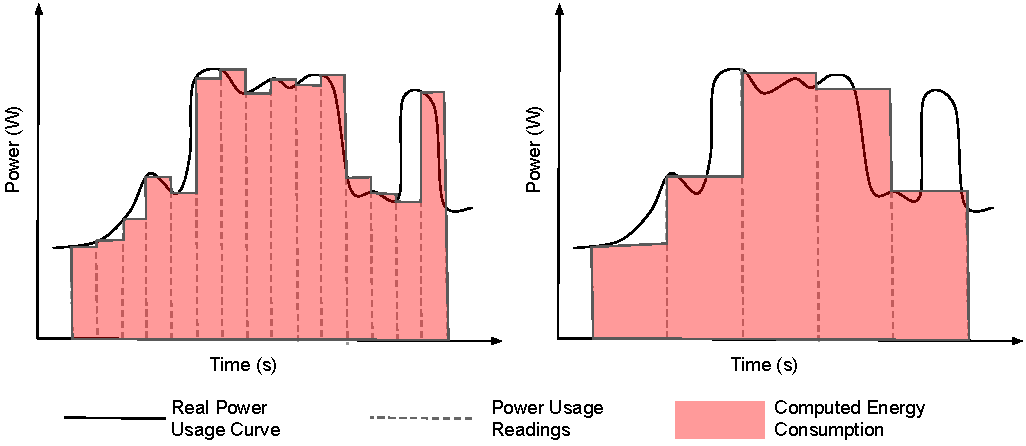
\includegraphics[width=0.49\textwidth]{other/figures/energy_measurment_schematic.pdf}
    \caption{Illustration of energy measurement from fine (left plot) and coarse (right plot) power reading intervals.}
    \label{fig:energy_illustration}
\end{figure}

\subsection{Other}
We use this section to capture derived metrics from the aforementioned metrics and discuss potential future metrics that can benefit the evaluation of compression techniques. 

\subsubsection{Improvement Ratio}
It is often that improvement ratio provided by a compression technique is reported in the literature ~\cite{He2018,Blalock2018,Menghani2023}. Two popular improvement ratios are \textit{compression ratio} and \textit{(theoretical) speedup ratio}.
%, given by equations \ref{compression_ratio} and \ref{speedup_ratio} respectively.
%
The speedup ratio refers to the reduction in computation time that can be achieved by using a compressed model, relative to the original uncompressed model. Typically calculated as a ratio between the computation time of the uncompressed model and the computation time of the compressed model (see Equation~\ref{compression_ratio}). When this speedup ratio computation is carried out using a non temporal metric e.g.(FLOPs, MAC) then it is referred to as \textit{theoretical speedup}.
%
% \subsubsection{Compression Ratio}
Similarly, \textit{compression ratio} is another derived metric based on size reduction of the model. It refers to the reduction in model size achieved by a compression technique, relative to the size of the original uncompressed model (see Equation~\ref{speedup_ratio}). 
%
We extend this further to include \textit{efficiency ratio} (see Equation~\ref{effeciency_ratio}), which aims at reporting improvement in energy consumption between the compressed and uncompressed models.
 
\begin{equation}
  \text{Speedup ratio} =   \frac{\text{original speed}}{\text{compressed speed}}
  \label{speedup_ratio}
\end{equation}

\begin{equation}
  \text{Compression Ratio} =   \frac{\text{original size}}{\text{compressed size}}
  \label{compression_ratio}
\end{equation}

\begin{equation}
  \text{Efficiency Ratio} =   \frac{\text{original energy consumption}}{\text{compressed energy consumption}}
  \label{effeciency_ratio}
\end{equation}

Reporting improvement ratios alone is not enough, as the ratio can be calculated using different metrics, for example one may calculate the compression ratio using disk size, whilst another can use parameters count, or CPU/GPU usage to calculate the compression ratio. Similarly, one may use inference latency, FLOPs, or MAC to compute speedup ratio.
%
Therefore when reporting improvement ratios, one need to outline what metrics were used in their computation to allow for reliable comparisons between different works. 

\subsubsection{Verification metrics}
Verification aims at providing confidence that the actual behaviour of a system matches the requirements and expected behaviour of the system~\cite{Chance_2020}. This is particularly important in deployment of machine learning models in safety critical applications.
%
Compressing after a model passed some verification processes may require tedious amounts of effort to rerun these verification evaluations.
% for different compression techniques and include it in the evaluation of the compression technique. 
%
Therefore, being able to ensure and quantify functional equivalence post compression is important and currently overlooked by the research community. Whilst the metrics discussed throughout this paper aim at evaluating different aspects of a neural network post compression, it is not clear how these metrics may be used to quantify functional equivalence in the context of verification. Further research can benefit in this direction.   
% functional equivalence, more research is required to investigate how these metrics may be used to quantify functional equivalence in the context of verification.  

\section{NetZIP Overview} \label{sec:NetZIP_overview}
% \subsection{Overview}
% We have put together a library containing all of the metrics reviewed in this paper and named it NetZIP. NetZIP 
%
We introduce NetZIP, a library based on PyTorch~\cite{paszke2017automatic} that provides a suite of metrics for evaluating the gains and losses in performance from different compression techniques.
%
The suite of metrics is based on the five evaluation categories reviewed in  section~\ref{sec:metrics}.
%
The goal of NetZIP is to provide a unified implementation of assessment metrics to ease and standardise the evaluation of compression techniques. Allowing for more reliable and unified comparisons across works by different researchers.
%
We provide a set of datasets and models to be used as baselines for running experiments, and help researchers get started.  
%
The NetZIP library may improve and and grow overtime, to include more baseline experiment and more metrics as research on neural network compression evolves. 
%
Figure~\ref{fig:Netzip} depicts an overview diagram of NetZIP showing how users may utilise NetZIP for their evaluation setup. 
%
Following lessons learnt from Blalock et.al.~\cite{Blalock2020}, one should compare models that have been compressed from the same uncompressed model; therefore we break NetZIP into three main stages: Train, Compress, and Compare. 

Using NetZIP, one can train a model from scratch or use a pretrained model and extend its training. 
%
The trained model is saved, and then in the ``Compress" stage this saved model is used as the starting uncompressed model for every different compression technique used. 
%
One can either use baseline compression methods available or program their own custom compression technique that they wish to evaluate. The different compressed models are saved and can be evaluated in the ``Compare" stage. 
%
In the ``Compare" stage, the user can select several options from the metrics suite to evaluate the compressed models against the uncompressed model and output a summary log file along with plots for each metric.% comparing the different compression techniques.% for each selected metric.
%
% Whilst one may utilise the ``Compare" stage in NetZIP to compare readily compressed models, we recommend to use the workflow constructed in the NetZIP library shown in Figure~\ref{fig:Netzip}, to ensure that any gains you get from compression is due to the compression technique used and not due to the different training or configuration settings.


\begin{figure}[h]
    \centering
    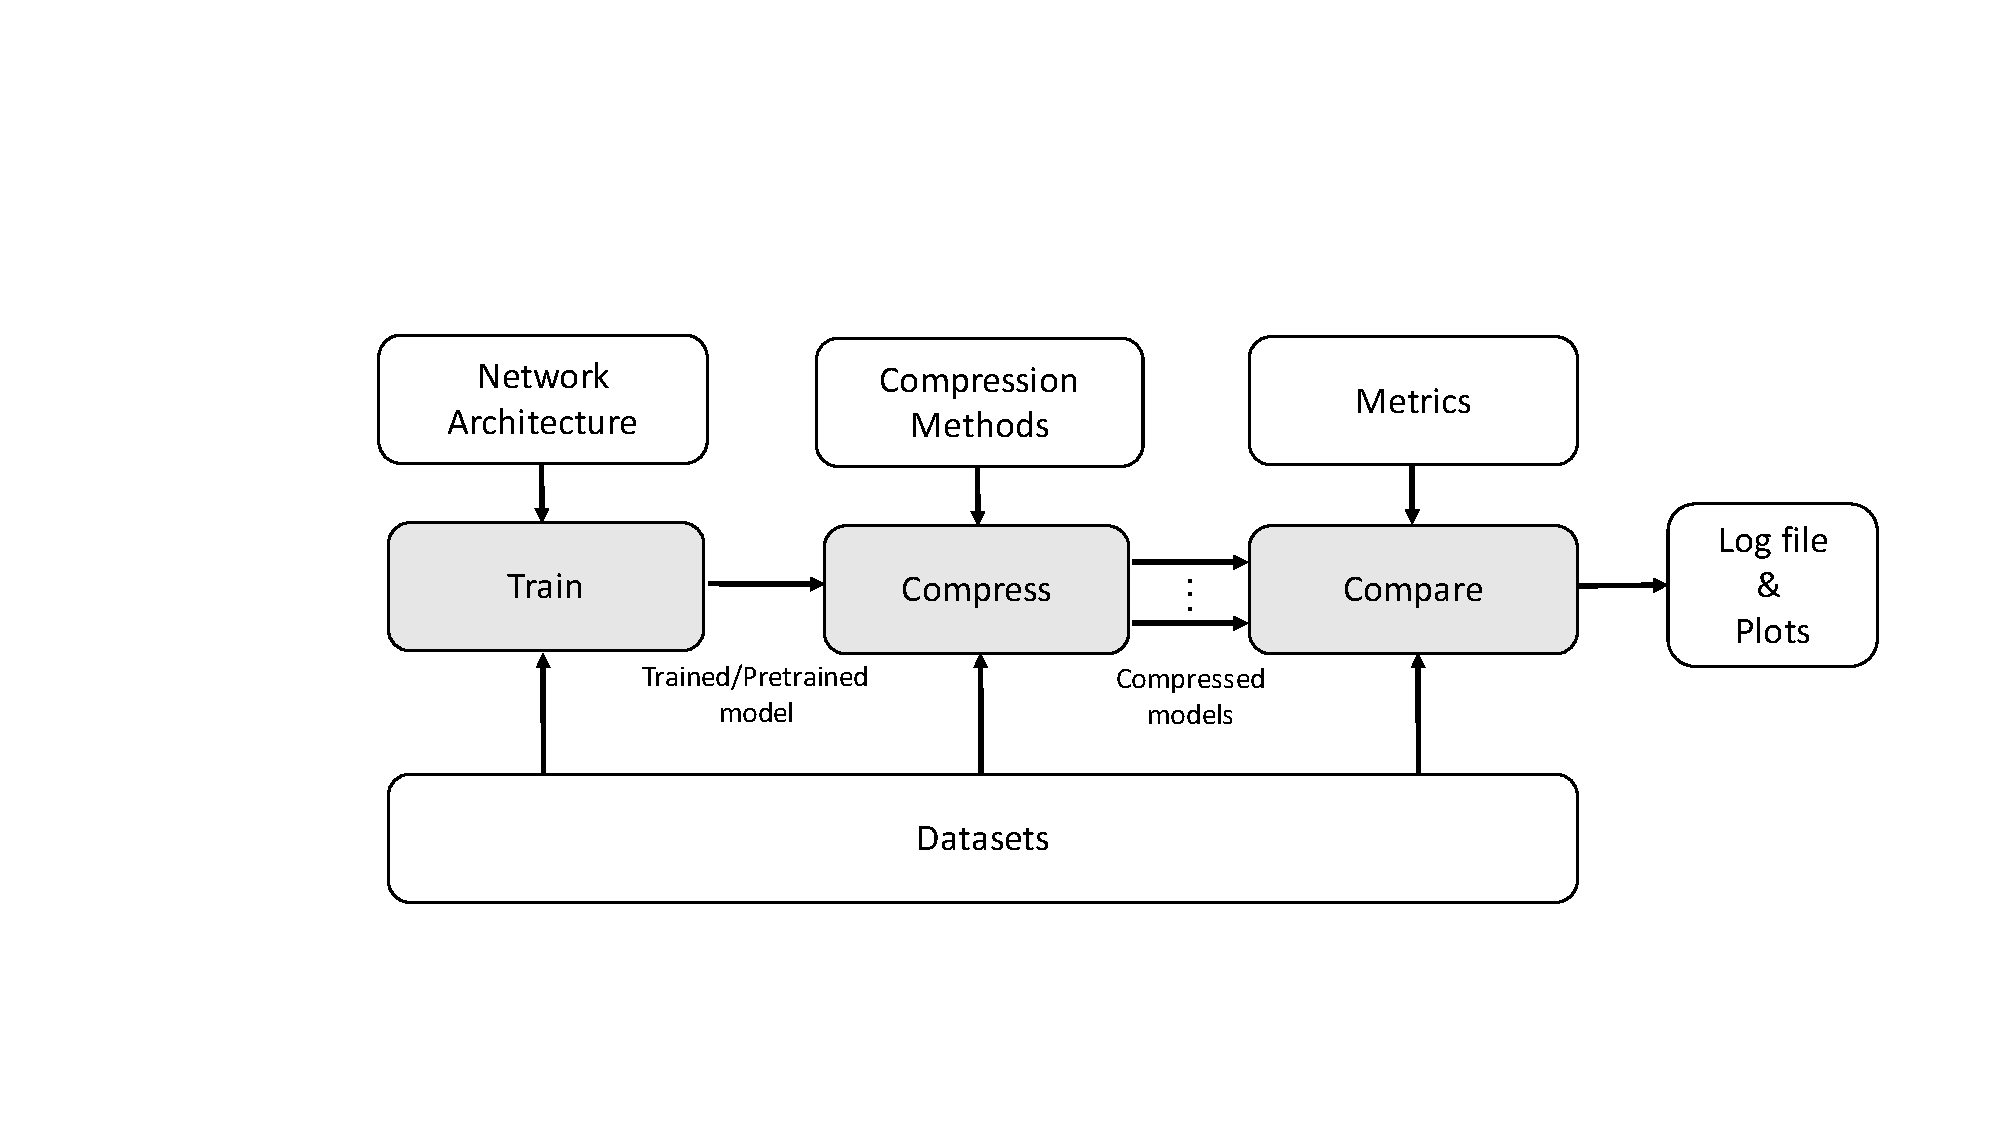
\includegraphics[width=0.49\textwidth]{other/figures/NetZIP_overview.pdf}
    \caption{NetZIP overview}
    \label{fig:Netzip}
\end{figure}



\section{Example Case Studies} \label{sec:casestudies}
We use three case studies to showcase the usage of metrics available in NetZIP. We break our case studies into three different themes: object classification, object detection, and edge devices. 
% We use the suite of metrics available in NetZIP to evaluate the effectiveness of different compression techniques in the three themes of our case studies.
%
Table~\ref{tab:casestudy_summary} shows a summary of the neural network architectures, datasets, compression techniques, and the machines used in our case studies. Table~\ref{tab:Hardware_summary} shows the machines hardware specifications. In all of our evaluations we eliminated the usage of GPU and used only CPU, to maintain fair availability of resources in our experiments, especially that some compression techniques implementations currently only operate on CPU. 

\begin{table*}[]
    \centering
    \begin{tabular}{| c  | c | c | c | c |} 
        \hline
        Theme & Network Architecture(s) & Datasets & Compression Techniques & Hardware  \\
        \hline        
        Object Classification  & ResNet18 & CIFAR10, ImageNet1k & PTQ, QAT, GUP$_R$, GUP$_{L1}$ & Laptop, PC \\ 
        Object Detection  & YOLOv5s & COCO  &  PTQ-TF  & Laptop  \\
        Embedded Systems  & YOLOv5s & COCO  & PTQ-TF  & RasPi 4 \\
        \hline
    \end{tabular}
    \caption{Case Studies Summary}
    \label{tab:casestudy_summary}
\end{table*}


\begin{table*}[]
    \centering
    \begin{tabular}{| l  | l | l | l |} 
        \hline
        Name & Product Name & Specifications & Operating System \\
        \hline        
        Laptop  & MSI GF65 THIN 3060  & 64GB RAM, NVIDIA 3060 & Linux Ubuntu 20.04.2 LTS (64-bit)\\ 
        PC  & Dell Alienware Desktop & 64GB RAM, NVIDIA 2080 & Linux Ubuntu 18.04.4 LTS (64-bit)\\
        RasPi 4  & Raspberry Pi 4 Model B & 4GB RAM &  Linux Ubuntu 22.04.2 LTS (64-bit) \\
        \hline
    \end{tabular}
    \caption{Hardware Specifications Summary.}% In all cases an Ubuntu Linux operating system was used.}
    \label{tab:Hardware_summary}
\end{table*}

% three different neural network architectures: VGG\cite{ref}, ResNet\cite{ref} and YOLO\cite{ref}. We use a number of different datasets in our case studies: CIFAR100\cite{ref}, TinyImagNet\cite{ref}, ImageNet\cite{ref}, COCO\cite{ref}.


% The case studies are broken into three themes, object classification, object detection

% networks 
% case studies to show case 
% There is a suite of example case studies implemented in NetZIP to guide users on how to utilise the evaluation metrics provided by NetZIP and also act as baselines for researchers experiments. 
% %
% We utilise this section to showcase the evaluation metrics reviewed on these different case studies. 

\begin{figure*}[]
    \centering
    \begin{subfigure}{0.19\textwidth}
        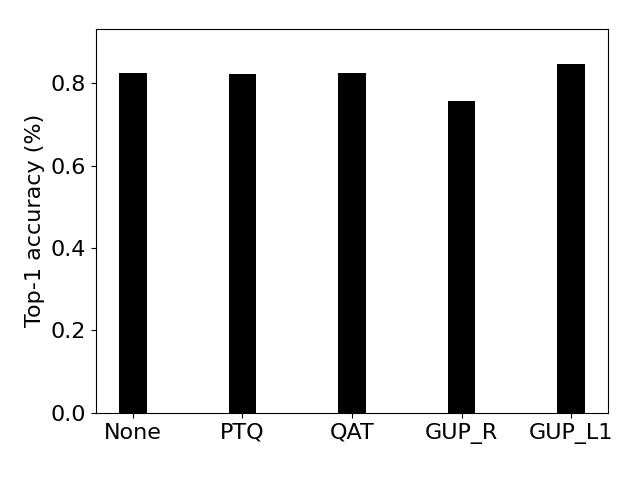
\includegraphics[width=1\textwidth]{other/figures/Resnet18_CIFAR10_Laptop/TOP1accuracy.png}
        \caption{Accuracy - Top1}
    \end{subfigure}
    \begin{subfigure}{0.19\textwidth}
        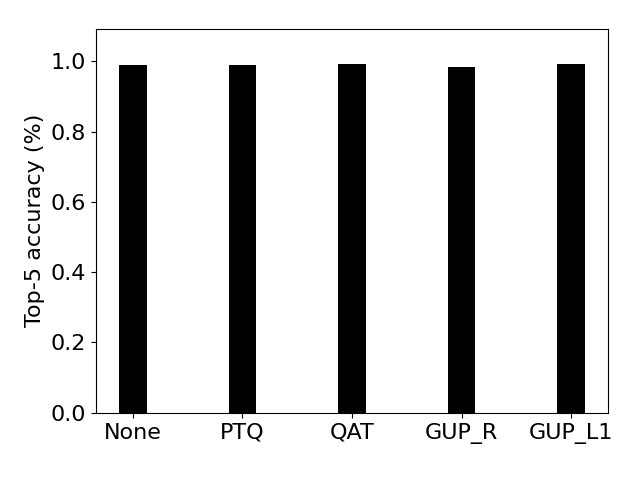
\includegraphics[width=1\textwidth]{other/figures/Resnet18_CIFAR10_Laptop/TOP5accuracy.png}
        \caption{Accuracy - Top5}
    \end{subfigure}
    \begin{subfigure}{0.19\textwidth}
        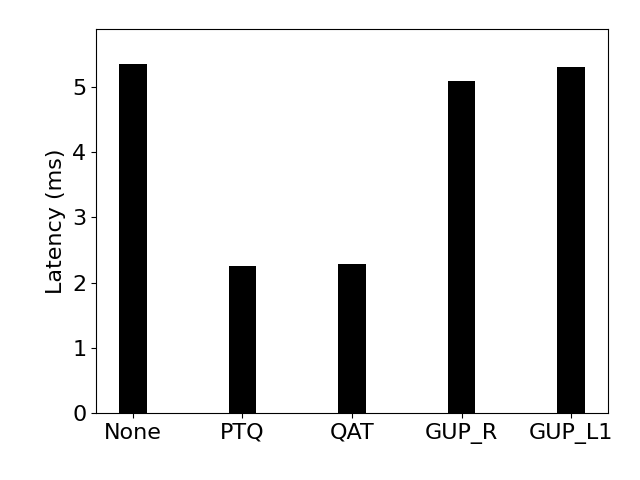
\includegraphics[width=1\textwidth]{other/figures/Resnet18_CIFAR10_Laptop/Latency.png}
        \caption{Speed - Latency}
    \end{subfigure}
    \begin{subfigure}{0.19\textwidth}
        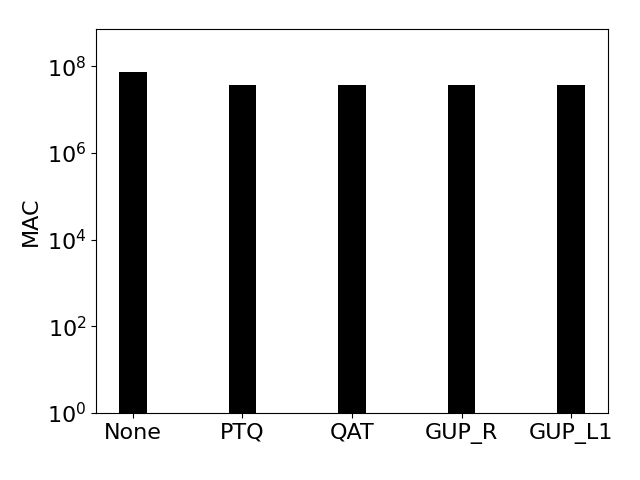
\includegraphics[width=1\textwidth]{other/figures/Resnet18_CIFAR10_Laptop/MAC.png}
        \caption{Speed - MAC}
    \end{subfigure}
    \begin{subfigure}{0.19\textwidth}
        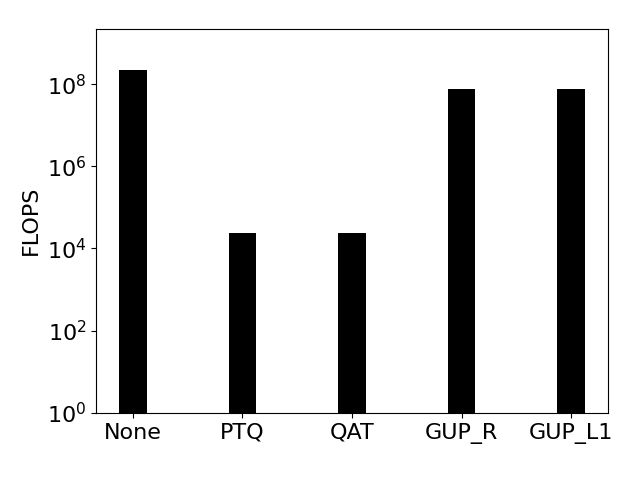
\includegraphics[width=1\textwidth]{other/figures/Resnet18_CIFAR10_Laptop/FLOPS.png}
        \caption{Speed - FLOPs}
    \end{subfigure}
    \begin{subfigure}{0.19\textwidth}
        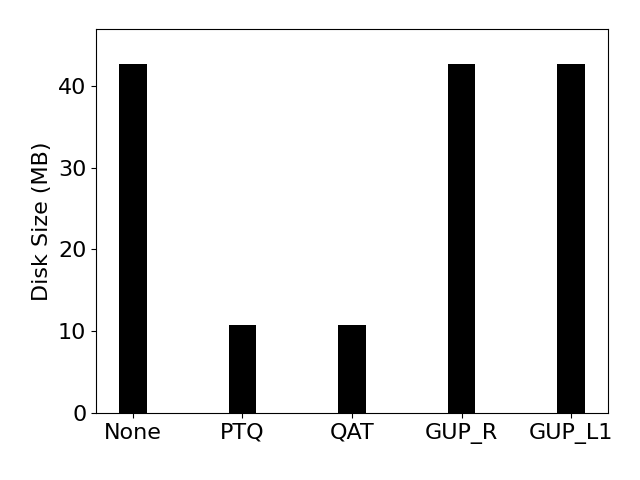
\includegraphics[width=1\textwidth]{other/figures/Resnet18_CIFAR10_Laptop/Size.png}
        \caption{Size - Disk Size}
    \end{subfigure}
    \begin{subfigure}{0.19\textwidth}
        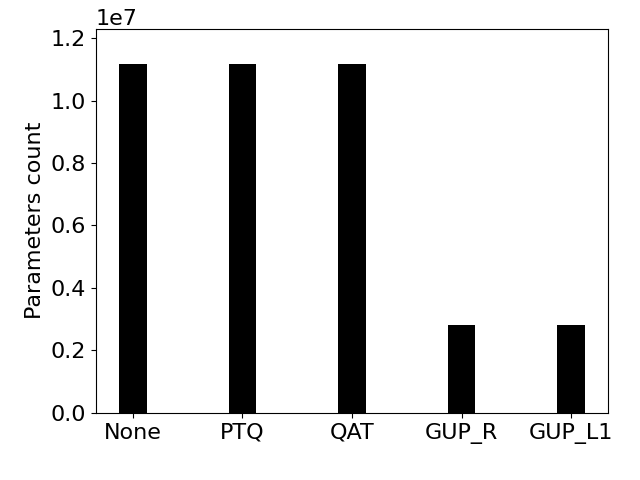
\includegraphics[width=1\textwidth]{other/figures/Resnet18_CIFAR10_Laptop/Parameters_count.png}
        \caption{Size - Params Count}
    \end{subfigure}
    \begin{subfigure}{0.19\textwidth}
        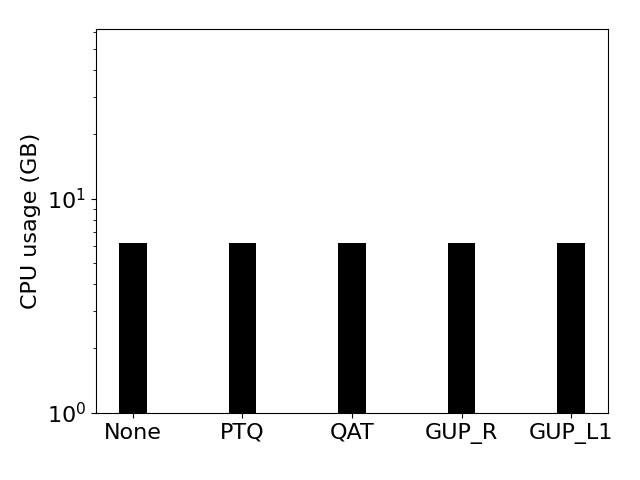
\includegraphics[width=1\textwidth]{other/figures/Resnet18_CIFAR10_Laptop/CPU_usage.png}
        \caption{Size - CPU usage}
    \end{subfigure}
    \begin{subfigure}{0.19\textwidth}
        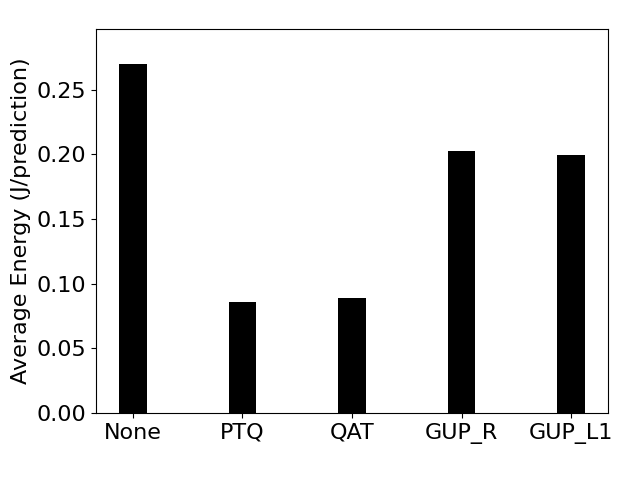
\includegraphics[width=1\textwidth]{other/figures/Resnet18_CIFAR10_Laptop/Energy.png}
        \caption{Energy -  Energy}
    \end{subfigure}
    \begin{subfigure}{0.19\textwidth}
        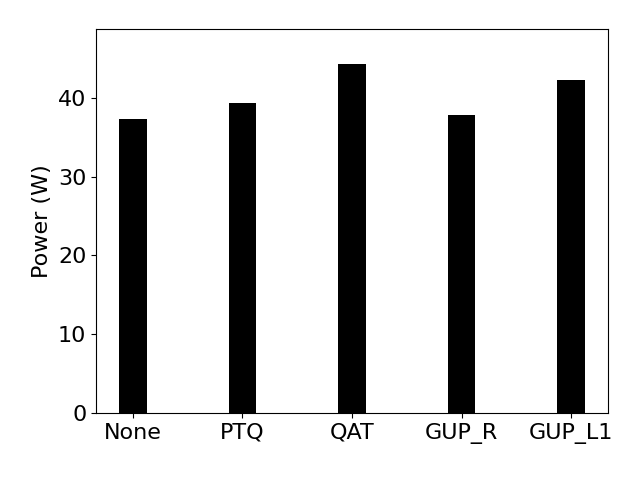
\includegraphics[width=1\textwidth]{other/figures/Resnet18_CIFAR10_Laptop/Power.png}
        \caption{Energy - Power}
    \end{subfigure}
    \caption{ResNet18 - CIFAR10 - Laptop}
    \label{fig:Resnet-cifar-laptop}
\end{figure*}

% \begin{figure*}[h]
%     \centering
%     \begin{subfigure}{0.19\textwidth}
%         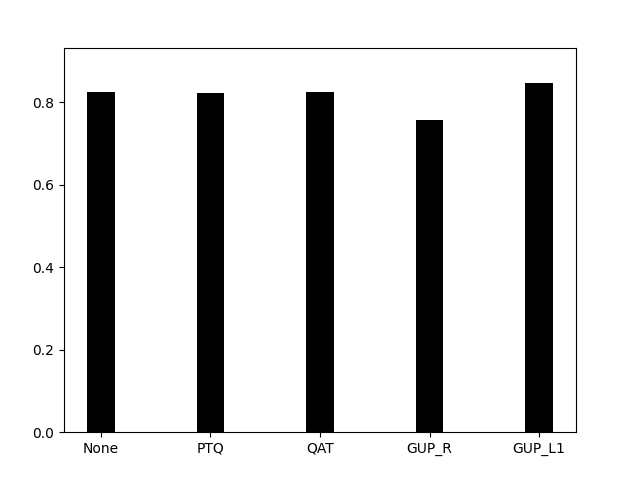
\includegraphics[width=1\textwidth]{other/figures/VGG11_TinyImageNet_Laptop/TOP1accuracy.png}
%         \caption{Accuracy - Top1}
%     \end{subfigure}
%     \begin{subfigure}{0.19\textwidth}
%         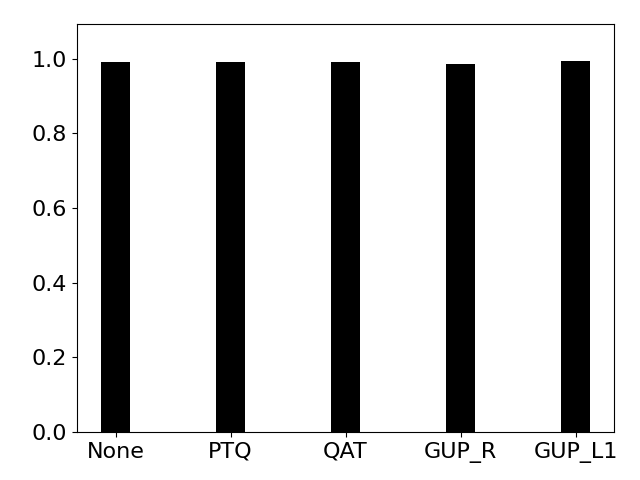
\includegraphics[width=1\textwidth]{other/figures/VGG11_TinyImageNet_Laptop/TOP5accuracy.png}
%         \caption{Accuracy - Top5}
%     \end{subfigure}
%     \begin{subfigure}{0.19\textwidth}
%         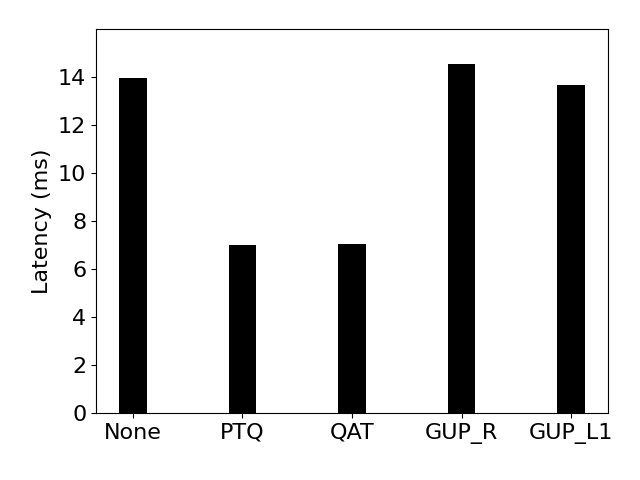
\includegraphics[width=1\textwidth]{other/figures/VGG11_TinyImageNet_Laptop/Latency.png}
%         \caption{Speed - Latency}
%     \end{subfigure}
%     \begin{subfigure}{0.19\textwidth}
%         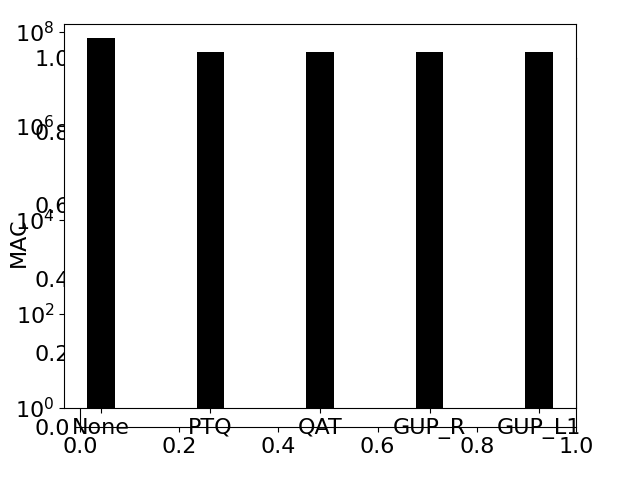
\includegraphics[width=1\textwidth]{other/figures/VGG11_TinyImageNet_Laptop/MAC.png}
%         \caption{Speed - MAC}
%     \end{subfigure}
%     \begin{subfigure}{0.19\textwidth}
%         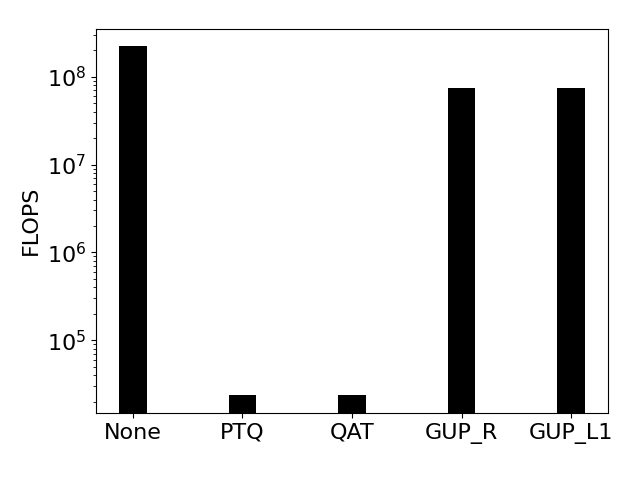
\includegraphics[width=1\textwidth]{other/figures/VGG11_TinyImageNet_Laptop/FLOPS.png}
%         \caption{Speed - FLOPs}
%     \end{subfigure}
%     \begin{subfigure}{0.19\textwidth}
%         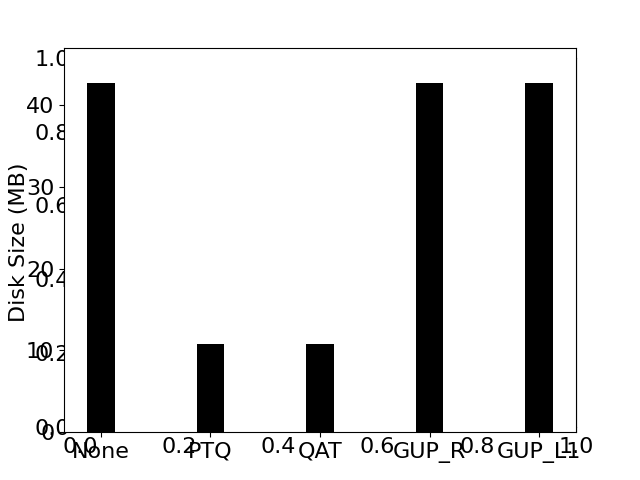
\includegraphics[width=1\textwidth]{other/figures/VGG11_TinyImageNet_Laptop/Size.png}
%         \caption{Size - Disk Size}
%     \end{subfigure}
%     \begin{subfigure}{0.19\textwidth}
%         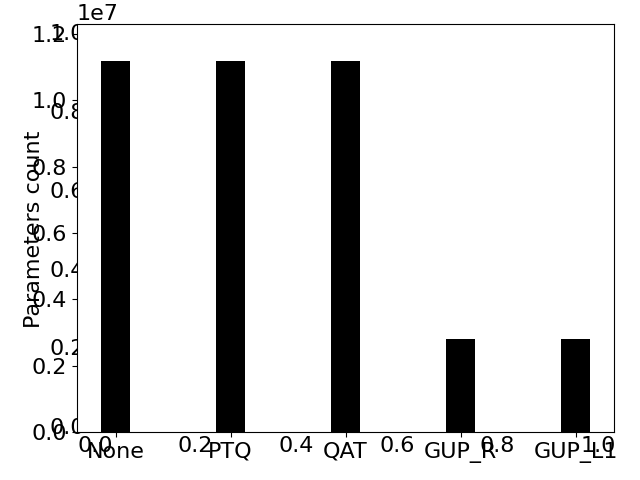
\includegraphics[width=1\textwidth]{other/figures/VGG11_TinyImageNet_Laptop/Parameters_count.png}
%         \caption{Size - Params Count}
%     \end{subfigure}
%     \begin{subfigure}{0.19\textwidth}
%         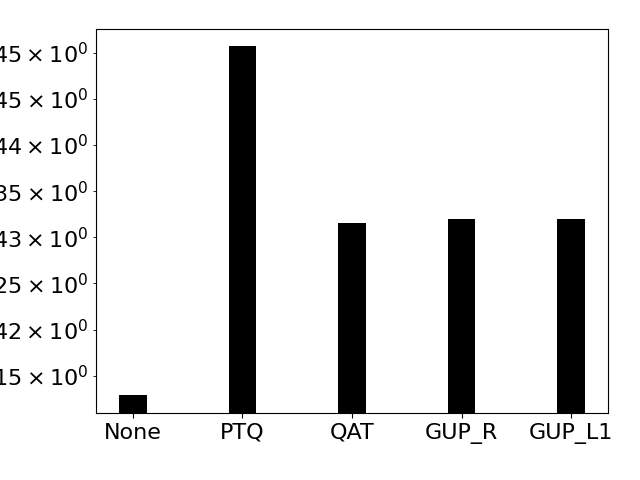
\includegraphics[width=1\textwidth]{other/figures/VGG11_TinyImageNet_Laptop/CPU_usage.png}
%         \caption{Size - CPU usage}
%     \end{subfigure}
%     \begin{subfigure}{0.19\textwidth}
%         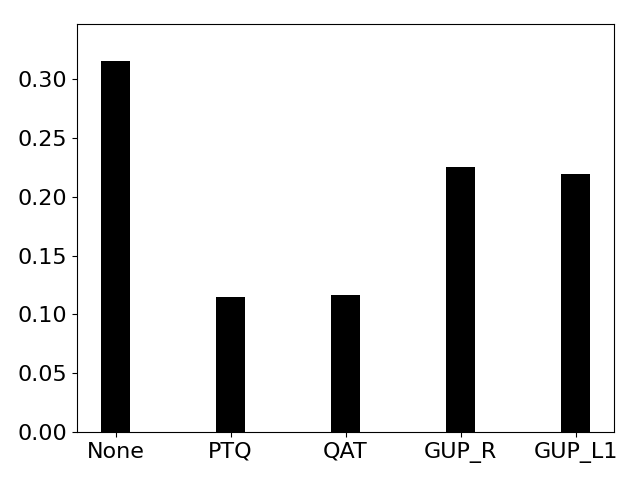
\includegraphics[width=1\textwidth]{other/figures/VGG11_TinyImageNet_Laptop/Energy.png}
%         \caption{Energy -  Energy}
%     \end{subfigure}
%     \begin{subfigure}{0.19\textwidth}
%         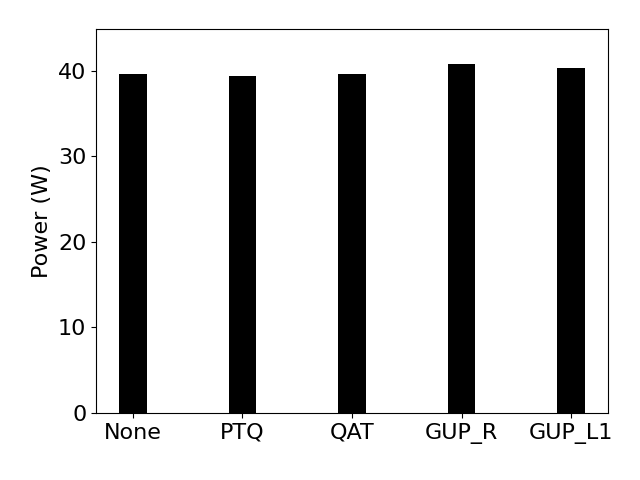
\includegraphics[width=1\textwidth]{other/figures/VGG11_TinyImageNet_Laptop/Power.png}
%         \caption{Energy - Power}
%     \end{subfigure}
%     \caption{VGG11 - TinyImageNet - Laptop}
% \end{figure*}

\begin{figure*}[]
    \centering
    \begin{subfigure}{0.19\textwidth}
        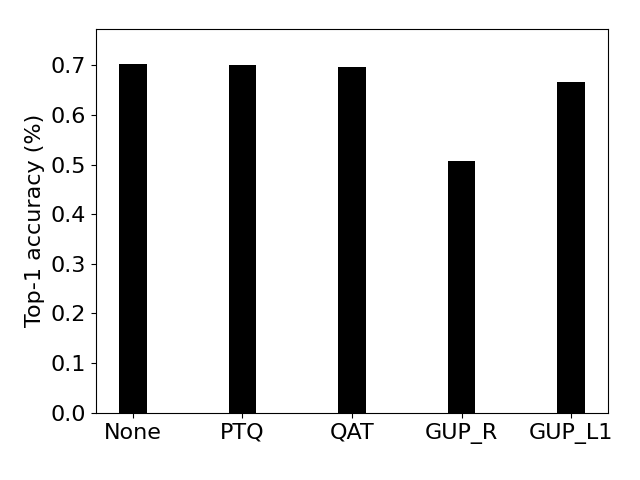
\includegraphics[width=1\textwidth]{other/figures/Resnet18_ImageNet1k_PC/TOP1accuracy.png}
        \caption{Accuracy - Top1}
    \end{subfigure}
    \begin{subfigure}{0.19\textwidth}
        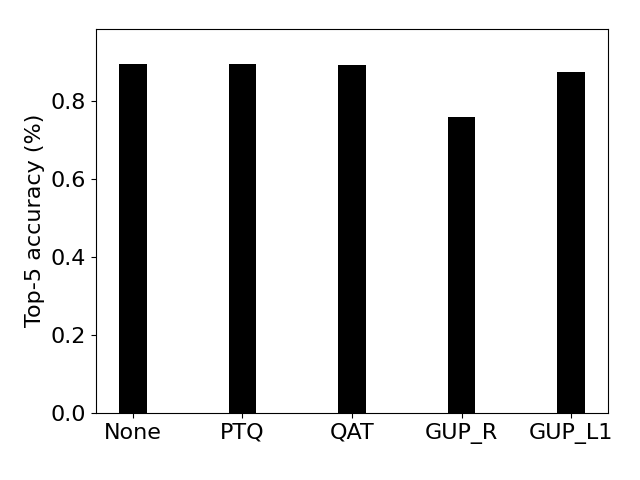
\includegraphics[width=1\textwidth]{other/figures/Resnet18_ImageNet1k_PC/TOP5accuracy.png}
        \caption{Accuracy - Top5}
    \end{subfigure}
    \begin{subfigure}{0.19\textwidth}
        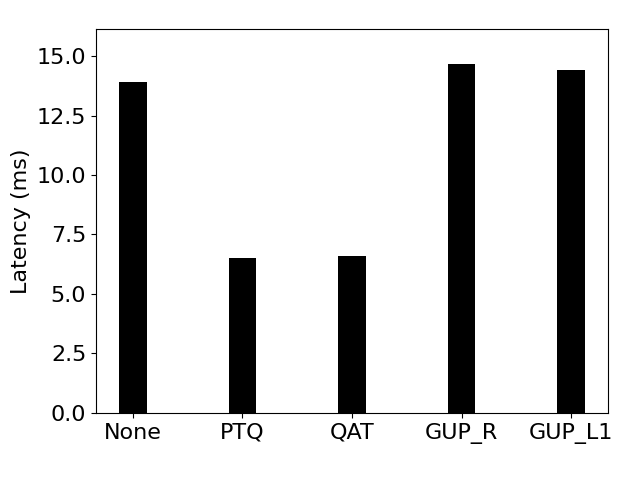
\includegraphics[width=1\textwidth]{other/figures/Resnet18_ImageNet1k_PC/Latency.png}
        \caption{Speed - Latency}
    \end{subfigure}
    \begin{subfigure}{0.19\textwidth}
        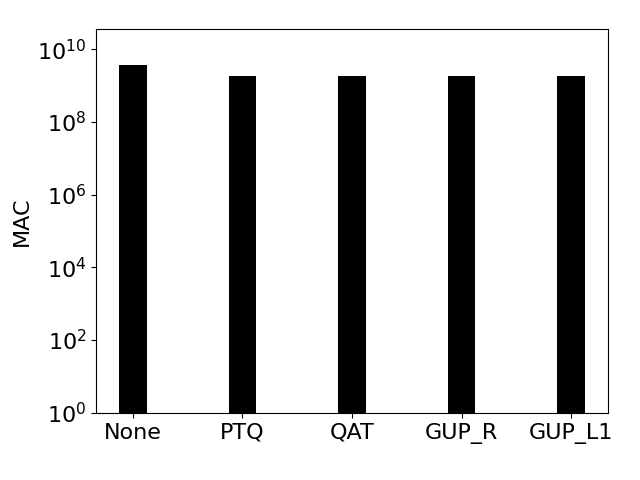
\includegraphics[width=1\textwidth]{other/figures/Resnet18_ImageNet1k_PC/MAC.png}
        \caption{Speed - MAC}
    \end{subfigure}
    \begin{subfigure}{0.19\textwidth}
        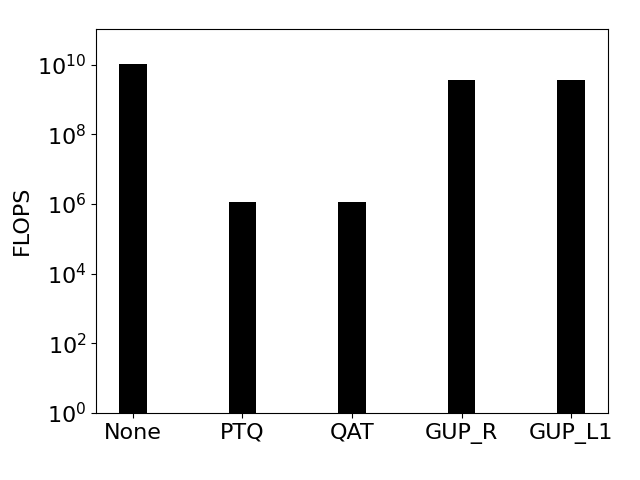
\includegraphics[width=1\textwidth]{other/figures/Resnet18_ImageNet1k_PC/FLOPS.png}
        \caption{Speed - FLOPs}
    \end{subfigure}
    \begin{subfigure}{0.19\textwidth}
        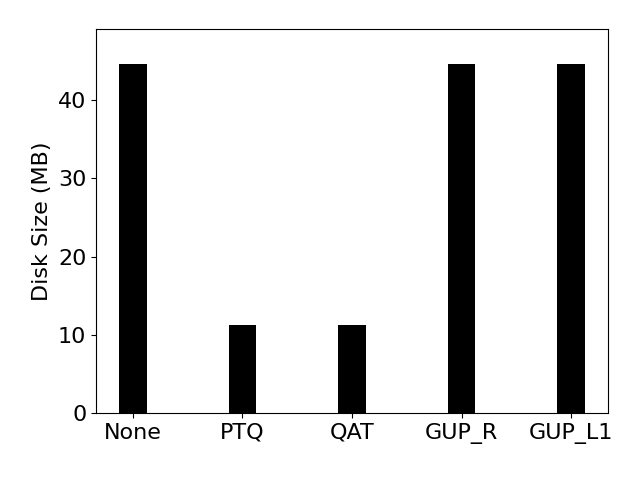
\includegraphics[width=1\textwidth]{other/figures/Resnet18_ImageNet1k_PC/Size.png}
        \caption{Size - Disk Size}
    \end{subfigure}
    \begin{subfigure}{0.19\textwidth}
        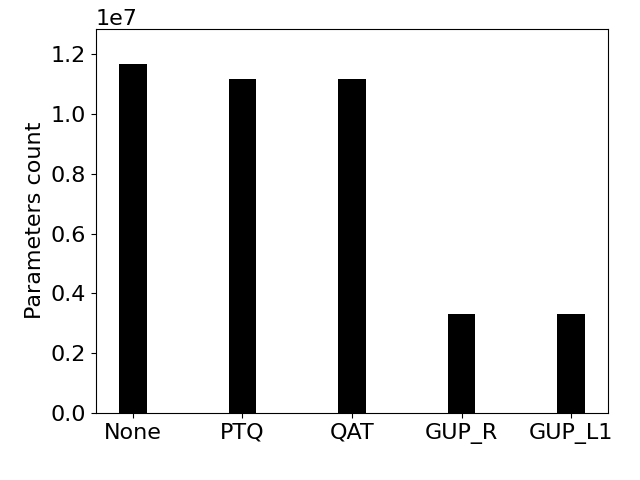
\includegraphics[width=1\textwidth]{other/figures/Resnet18_ImageNet1k_PC/Parameters_count.png}
        \caption{Size - Params Count}
    \end{subfigure}
    \begin{subfigure}{0.19\textwidth}
        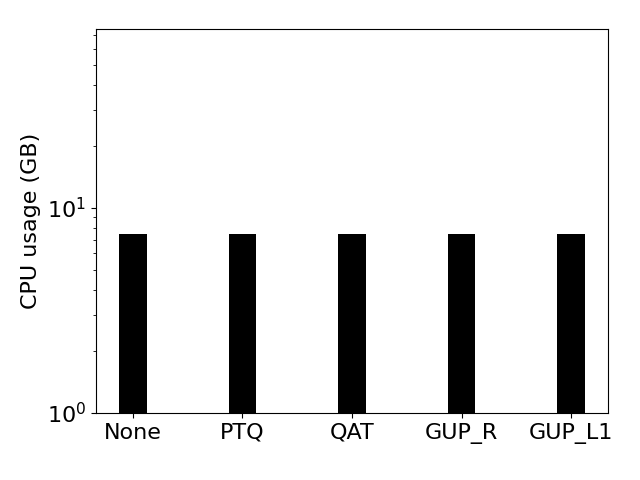
\includegraphics[width=1\textwidth]{other/figures/Resnet18_ImageNet1k_PC/CPU_usage.png}
        \caption{Size - CPU usage}
    \end{subfigure}
    \begin{subfigure}{0.19\textwidth}
        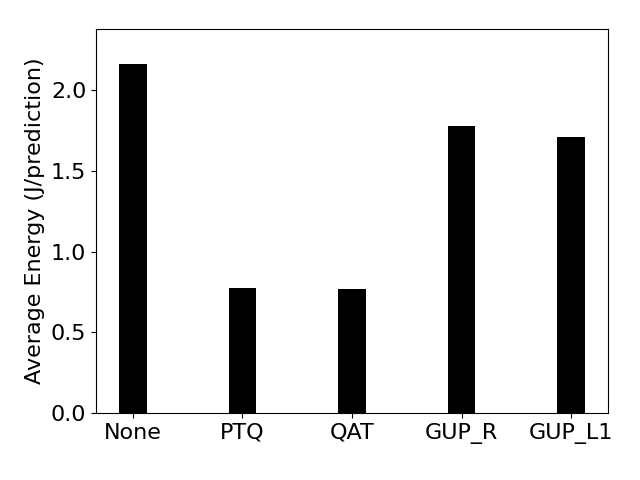
\includegraphics[width=1\textwidth]{other/figures/Resnet18_ImageNet1k_PC/Energy.png}
        \caption{Energy -  Energy}
    \end{subfigure}
    \begin{subfigure}{0.19\textwidth}
        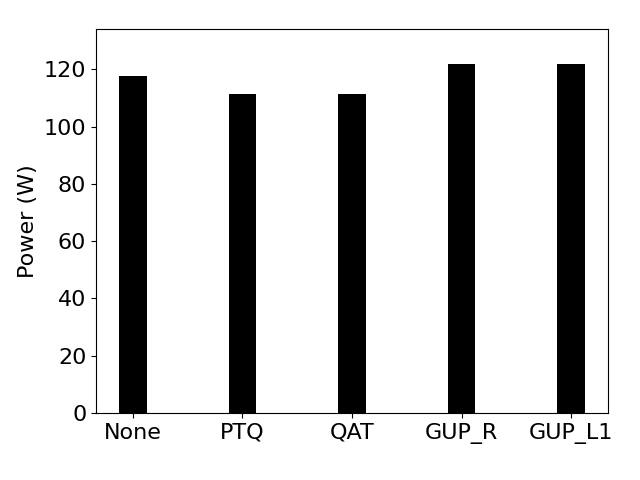
\includegraphics[width=1\textwidth]{other/figures/Resnet18_ImageNet1k_PC/Power.png}
        \caption{Energy - Power}
    \end{subfigure}
    \caption{ResNet18 - ImageNet1k - PC}
    \label{fig:Resnet-imagenet-pc}
\end{figure*}

\begin{figure*}[]
    \centering
    \begin{subfigure}{0.19\textwidth}
        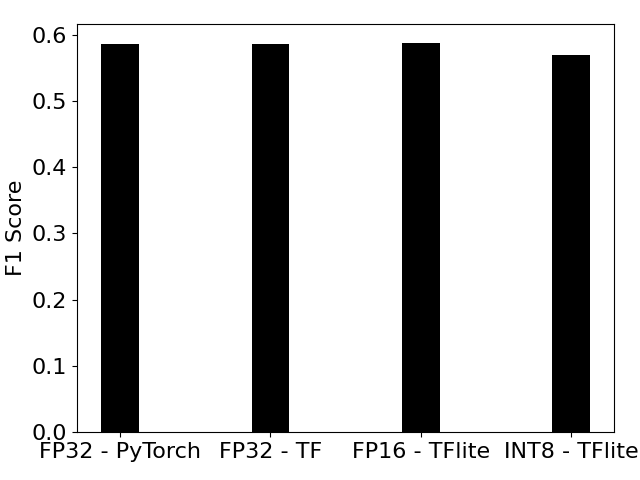
\includegraphics[width=1\textwidth]{other/figures/YOLOv5s_COCO_Laptop/F1score.png}
        \caption{Accuracy - F1 Score}
    \end{subfigure}
    \begin{subfigure}{0.19\textwidth}
        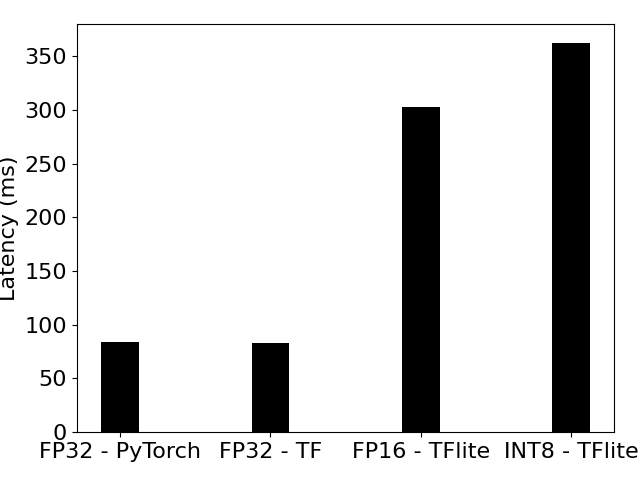
\includegraphics[width=1\textwidth]{other/figures/YOLOv5s_COCO_Laptop/Latency.png}
        \caption{Speed - Latency}
    \end{subfigure}
    \begin{subfigure}{0.19\textwidth}
        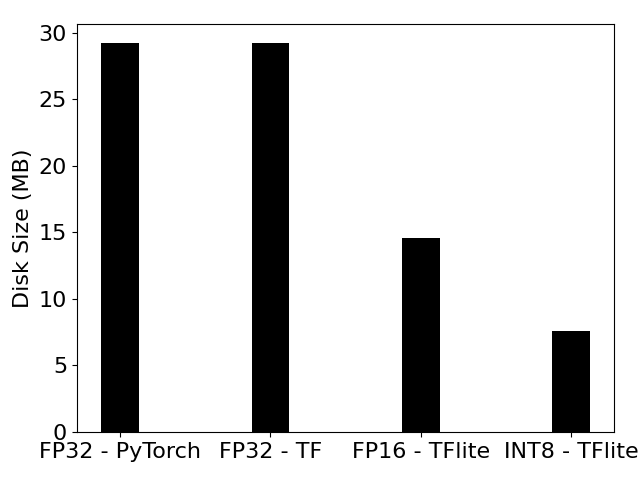
\includegraphics[width=1\textwidth]{other/figures/YOLOv5s_COCO_Laptop/Size.png}
        \caption{Size - Disk Size}
    \end{subfigure}
    \begin{subfigure}{0.19\textwidth}
        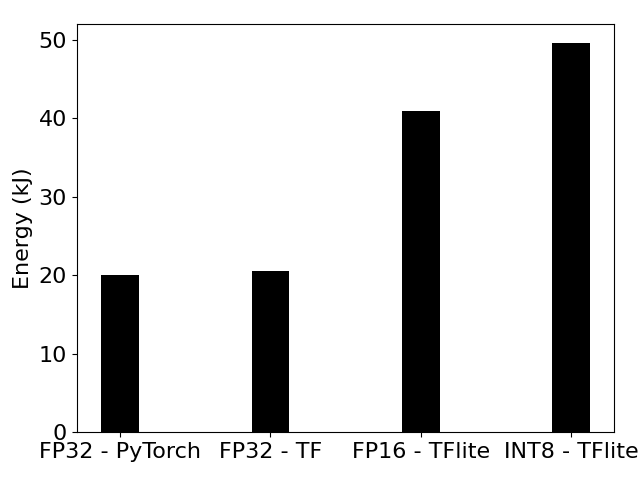
\includegraphics[width=1\textwidth]{other/figures/YOLOv5s_COCO_Laptop/Energy.png}
        \caption{Energy - Energy}
    \end{subfigure}
    \begin{subfigure}{0.19\textwidth}
        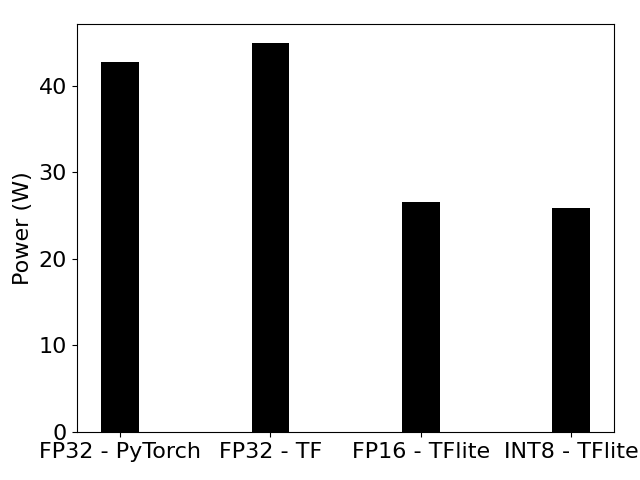
\includegraphics[width=1\textwidth]{other/figures/YOLOv5s_COCO_Laptop/Power.png}
        \caption{Energy - Power}
    \end{subfigure}
    \caption{YOLOv5s - COCO - Laptop}
    \label{fig:yolo-coco-laptop}
\end{figure*}

\begin{figure*}[]
    \centering
    \begin{subfigure}{0.19\textwidth}
        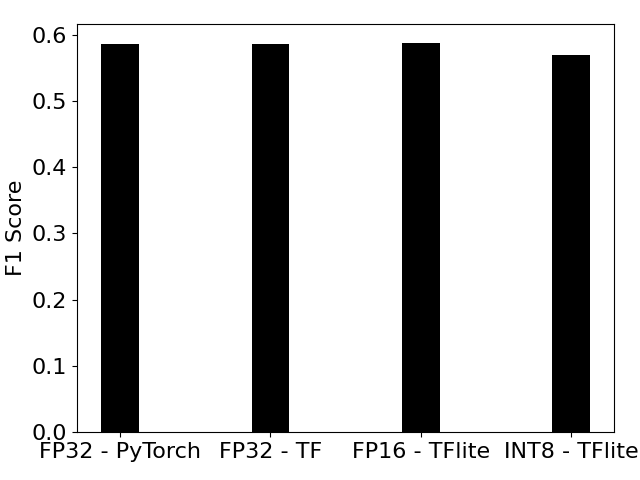
\includegraphics[width=1\textwidth]{other/figures/YOLOv5s_COCO_RasPi/rasPI_f1score_v2.png}
        \caption{Accuracy - F1 Score}
    \end{subfigure}
    \begin{subfigure}{0.19\textwidth}
        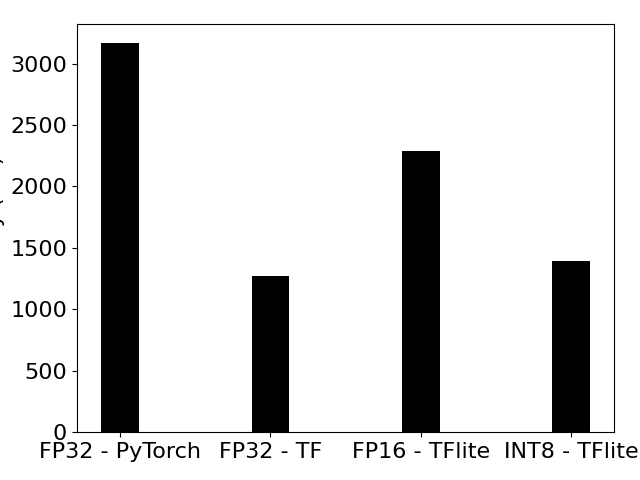
\includegraphics[width=1\textwidth]{other/figures/YOLOv5s_COCO_RasPi/rasPI_latency_v2.png}
        \caption{Speed - Latency}
    \end{subfigure}
    \begin{subfigure}{0.19\textwidth}
        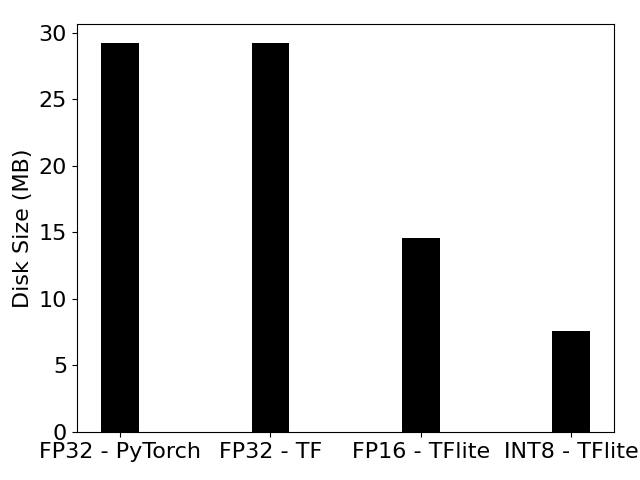
\includegraphics[width=1\textwidth]{other/figures/YOLOv5s_COCO_RasPi/rasPI_size_v2.png}
        \caption{Size - Disk Size}
    \end{subfigure}
    \begin{subfigure}{0.19\textwidth}
        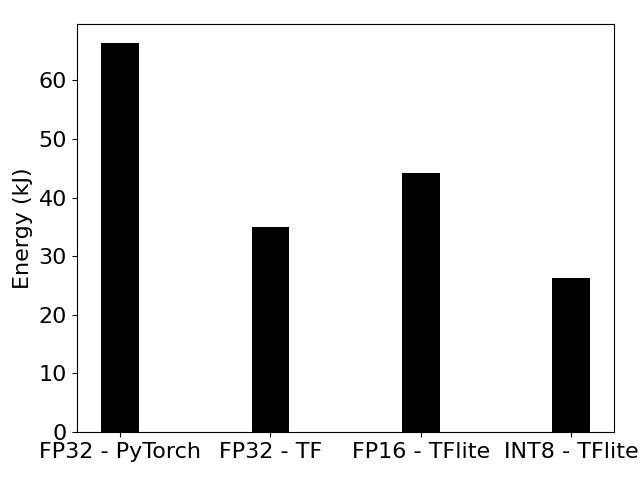
\includegraphics[width=1\textwidth]{other/figures/YOLOv5s_COCO_RasPi/rasPI_energy_v2.png}
        \caption{Energy - Energy}
    \end{subfigure}
    \begin{subfigure}{0.19\textwidth}
        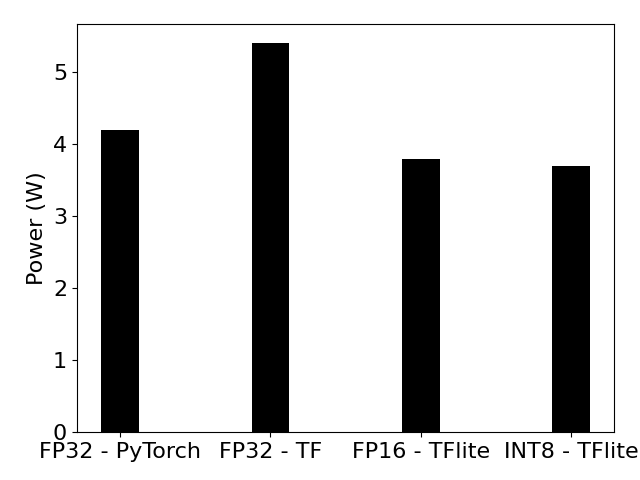
\includegraphics[width=1\textwidth]{other/figures/YOLOv5s_COCO_RasPi/rasPI_power_v2.png}
        \caption{Energy - Power}
    \end{subfigure}
    \caption{YOLOv5s - COCO - Raspberry Pi}
    \label{fig:yolo-coco-raspeberrypi}
\end{figure*}


\subsection{Object Classification}
The first theme in our case studies is for object classification. 
%
We used four compression techniques, two based on quantisation and two based on pruning: 1) Post Training Quantisation (PTQ), 2) Quantisation Aware Training (QAT), 3)  Global Unstructured Random Pruning (GUP$_R$) and 4) Global Unstructured L1-norm Pruning (GUP$_{L1}$) i.e. components with lowest values get pruned. 
%
% We have run experiments using
We show experiments run using ResNet18~\cite{he2015deep} architecture
%and VGG11\cite{} 
on CIFAR10~\cite{krizhevsky2009learning}
%, TinyImageNet\cite{} 
and ImageNet1k~\cite{imagenet_cvpr09} datasets. 
% However we only show results based on ResNet18 here due to space limitations.

Figures~\ref{fig:Resnet-cifar-laptop} and \ref{fig:Resnet-imagenet-pc} shows matrix plots output from NetZIP using different metrics for CIFAR10 and ImagNet1k datasets respectively.
%
Each plot shows a different metric. The x-axis shows the compression method and the y-axis shows the output value of the assessment metric. 

For PTQ, QAT and GUP$_{L1}$ compression techniques the accuracy is maintained more or less the same for both CIFAR10 and ImageNet1k, whilst for GUP$_{R}$ the drop in accuracy is clearly more significant.
%
For speed, quantisation techniques provide a clear improvement in inference latency. However, the speed improvement can not be noticed using any of the speed metrics for pruning. This is due to the issue discussed earlier with current pruning implementations where the pruned parameters are zeroed but not removed from the architecture. Removing the pruned parameters can output errors from the architecture therefore, removing pruned parameters currently relies on custom processes dependent on the architecture. However there are efforts being made in automating the removal of pruned parameters from models e.g.~\cite{fang2023depgraph}. 
%
Alternatively, since speed metrics MAC and FLOPs have are related to parameters count, one may be able to deduce an expected improvement in speed when the number of non-zero parameters are counted, as shown by the ``Params Count" metric plot. Observing the parameters count, it can be seen that there is a significant improvement in speed expected to happen once pruned parameters are removed. %Based on this a similar improvement is also expected to occur to the disk size of the model.% so as to the size of the model. 

Inspecting model size metrics, the disk size metric shows that quantisation decreases the model size by a quarter, whilst pruning does not. This again due to the same problem discussed with zero parameters are not removed from the model. Using parameters count of non-zero parameters, again can be used in this case to show the expected decrease in disk size occupied by the pruned model. Additionally, no improvement was noticed in CPU usage by compressed models.
%
% Another aspect of size is the resources CPU usage size. There are no significant changes noticeable from the CPU usage plot as a result of compression. 

For Energy metrics, the average power seems to hold with little variations.%, possibly due to difficulty controlling operation system background processes involved in big computers like laptops and PCs. 
However for the average energy used to output a prediction the quantisation techniques provided a clear improvement, with the pruning techniques providing still a decrease in energy consumption even though the pruned parameters are not removed from the model. Interestingly, zeroing parameters seems to still provide more efficiency in terms of energy consumption. 


\subsection{Object Detection}
Beyond object classification, we run experiments for object detection using YOLOv5s~\cite{Jocher_YOLOv5_by_Ultralytics_2020} on COCO~\cite{lin2015microsoft} dataset.
%
We use the compression methods already integrated within the YOLOv5 repository~\cite{Jocher_YOLOv5_by_Ultralytics_2020} in this case study, which are limited to post training quantisation using TensorFlow lite (TFlite) to FP16 and INT8 numerical representations.
%
Figure~\ref{fig:yolo-coco-laptop} shows plots evaluating the effectiveness of compression in each of the four main categories of metrics that we have discussed previously. 
%
For accuracy, no significant changes in performance can be spotted from the bar plot. 
%
However, interestingly the inference latency has increased with compression. 
%
The size of the model has decreased as expected so as the power consumption, but the energy consumption for outputting predictions has increased with quantisation.
%
The reason why the latency and the energy consumption increase after quantisation may be attributed to the different library implementations between our uncompressed base lines (FP32-PyTorch and FP32-TensorFlow) and the TensorFlow lite quantisation. 
%
Even between quantisation from FP16-TFlite to INT8-TFlite the speed and energy performance worsens, which is counter-intuitive. 
%
We speculate that this may be limited by configurations in the operation system that may need alteration to maximise efficiency of TFlite models. 
%
Investigating these speculations are beyond the scope of this paper, however it is important that these factors are investigated further in real life applications.

% - YOLO ~\cite{Jocher_YOLOv5_by_Ultralytics_2020} on laptop (F1 Score, Network Size, Latency, Energy)
\subsection{Edge Devices}
We distinguish that the real benefit of compression in neural networks is to allow their deployment on real-time systems where inference time and energy consumption are key. Therefore we extend the YOLOv5s case study to run on a raspberry pi.
%
One thing to note is that raspberry pi does not have an intel CPU, which is key for the {\tt pyrapl} function for measuring energy to work. Instead we used a SIGLENT SPD3303X Programmable power supply to measure the energy consumption. 
%
Figure~\ref{fig:yolo-coco-raspeberrypi} shows the output of this experiment.
%
In this setup, the benefits of using TFlite models is prevalent compared to the experiment using a Laptop shown in Figure~\ref{fig:yolo-coco-laptop}.
%
Yet, interestingly on the raspberry pi the TensorFlow implementation using FP32 still had better speed compared to TensorFlow lite (TFlite) 8 bit integer numerical representation. 
%
However, the energy consumption of the TFlite INT8 was the most energy efficient. This observation is very interesting as one may expect the INT8 implementation to be both quicker and more energy efficient. 
%
Field et.al.~\cite{Field2014} reported a similar observation, where shorter bits save more energy but take more execution time than longer bit representations. 
%
This may perhaps be resolved through reconfiguration of hardware, however, it is beyond the scope of this paper to investigate technically how this can be achieved.

% Paper on energy transparency to support the case that longer bits tend to be quicker than shorter bits \cite{Field2014}, however shorter bits save more energy.


% yolo quantisation vs pruning

% \section{Discussion} \label{sec:Discussion}

% - Importance in security applications where processing has to be done on board and hence energy consumption and performance are key for effective functioning of the system.

% - Metrics provided can serve in domain of evaluating the trustworthiness of a system as energy can play a major role [trustworthiness paper (discussing spider web trustworthiness mapping)] 

% - In our context of metrics for evaluating compression, not being able to remove the pruned parameters stops us from evaluating size and speed gains from compression after pruning. To overcome this problem we use sparsity level to derive metrics for measuring size and speed of pruned models. These can be seen as helpful metrics either for evaluating the model before one committing to designing a manual-case-specific process for removing pruned parameters, or as temporary metrics for evaluating the effectiveness of pruning until research advances to generalising and automating the removal of zero parameters from different neural network architectures.   


\section{Conclusions and Future Works} \label{sec:Conclusions}
In this paper we have provided a review of evaluation metrics for neural networks compression, with the aim of standardising evaluation of neural network compression.
%
The metrics are grouped into five categories: Accuracy, Speed, Size, Energy, and Other.
The metrics reviewed were implemented and included in a compression bench library and named NetZIP, available publicly.
%
We used NetZIP to demonstrate the usage of most metrics reviewed in three different case studies focusing on object classification, object detection, and edge devices.

Throughout the development of this work we used Quantisation and Pruning as the compression strategies on a limited number of neural network architectures. A future work is to expand NetZIP to include other compression strategies (e.g. Knowledge Distillation, Tensor Decomposition) and more neural network architectures.
%
Expanding to natural language processing (NLP) applications is another area for expanding in future works.
% Additionaly, we mainly focussed on vission aplications in our work and scope for expanding to other applications e.g. Natural langale preocessing (NLP) 

Carrying this work out we have identified other interesting areas of research that seem to not have attracted a lot researchers interests. 
%
Currently, pruning techniques only zero parameters but pruned parameters are not removed from the model architecture automatically, as removal of parameters from an architecture can result in errors.
%
There is need for developing model agnostic techniques for removal of pruned parameters.
%
Additionally, there is still scope for development of new metrics focused on  verification transferability pre- and post-compression.
%
Furthermore, there is need for doing more feasibility studies for utilisation of compressed models on edge devices. 
% - Verification transferability pre- and post-compression metric. 
%
% How can information theory be used to quantify info lost and hence quantify verification transferability.
%
% - Expand to knowledge distillation and tensor decomposition compression techniques.
%
% - Expanding to natural language processing (NLP) applications.



\section{Acknowledgements}
The work has been funded by the Thales Bristol Partnership in Hybrid Autonomous Systems Engineering (T-B PHASE).
%
This paper is based upon work from the COST Action no. CA19135 ``Connecting Education and Research Communities for an Innovative Resource Aware Society (CERCIRAS)", supported by the European Commission through the European Cooperation in Science and Technology (COST) Association.

